\documentclass[12pt]{article}
\usepackage[pdftex]{graphicx}

\setlength{\oddsidemargin}{-0.25in}
\setlength{\evensidemargin}{-0.25in}
\setlength{\topmargin}{-0.25in}
\setlength{\headheight}{0in}
\setlength{\headsep}{0in}
\setlength{\textwidth}{7in} % Width of text on page
\setlength{\textheight}{9in} % Height of the body of page (excluding foot, head)
\setlength{\columnwidth}{\textwidth}
\setlength{\marginparwidth}{0pt} % Marginal comments
\setlength{\marginparsep}{0pt} % Marginal comments
\setlength{\parindent}{0.3in} % Indentation at begin of paragraph 
%\setlength{\parskip}{0.125in} % Extra vertical space between paragraphs
%\raggedright

\def\Mg{Mg$^{2+}$~}
\def\Ba{Ba$^{2+}$~}
\def\Cd{Cd$^{2+}$~}
\def\Ca{Ca$^{2+}$~}
\def\Na{Na$^+$~}
\def\K{K$^+$~}
\def\Cl{Cl$^-$~}
\def\uM{$\mu$M~}
\def\s{$\sec^{-1}$~}
\def\phos{${\rm photons}\,\mu {\rm m}^{-2}$}
\def\phoflux{${\rm photons}\,\mu {\rm m}^{-2} \,{\rm sec}^{-1}$}
\def\Lphos{photoisomerizations$/$sec$/$L cone}
\def\CO2{CO$_2$~}
\def\O2{O$_2$~}
\def\on{{\sc on}~}
\def\off{{\sc off}~}
\def\onoff{{\sc on/off}~}
\def\bi{\begin{itemize}}
\def\ei{\end{itemize}}
\def\i{\item}
\def\be{\begin{enumerate}}
\def\ee{\end{enumerate}}
\def\GCAPKO{GCAP$^{-/-}$}
\def\GCAPHET{GCAP$^{+/-}$}
\def\ArrKO{Arr$^{-/-}$}
\def\ArrHET{Arr$^{+/-}$}
\def\RKKO{GRK1$^{-/-}$}
\def\RKHET{GRK1$^{+/-}$}
\def\CVArea{CV$_{area}$~}
\def\tpeakratio{$t_{peak, \sigma^2} / t_{peak, m}$}

\begin{document}

\baselineskip 18pt

\leftline{\bf Todo: analysis/conceptual}

\be

\i{We are ignoring feedback --- is this ok?}

\i{Can we ignore saturation at channels?  There seems to be decent evidence against it, and it is hard to cleanly implement.}

\i{Clarify argument about \CVArea for stochastic transducin model in methods --- some of this can be taken from Dan's notes on subject.  Make sure consistent with how simulations are being done.}

\i{Decide how many different saturation models to consider: (1) Rh; (2) cumulative T; (3) instantaneous transducin}

\i{Run likelihood models for various combinations of noise from rhodopsin and transducin}

\i{How do we handle Rh* inactivation time constant in cases where inactivation not exponential?}

\i{Make schematic figure showing parameters used from time-dependent variance}

\i{Other comparisons for likelihood analysis?}

\i{Add table with experimental parameters and model results}

\i{Include more raw \GCAPKO data since that is new}

\i{How biased are single photon responses - i.e. are these cells out of the norm?  Check Pepperberg time constants if we have them on cells from which we have isolated singles.  Any other parameters too.}

\i{GCAP knockout feedback analysis}

\i{wt/1P comparison with coexpression}

\ee


\vfill\eject
\section{Introduction}

The ability of rod photoreceptors to respond to single photons provides an unparalleled opportunity to study how signals originating from single G-protein coupled receptors (GPRCs) are controlled.  The resulting electrical responses show much less variability than expected from other familiar signals controlled by single molecules --- such as the charge flowing through an ion channel during a single opening.  

The activity of a single light-activated rhodopsin molecule is amplified by a G-protein cascade in the rod outer segment to produce an electrical response.  Rhodopsin catalytically activates the G-protein transducin, which in turn activates a cGMP phosphodiesterase.  These initial steps in the transduction process take place on the surface of membrane discs in the rod outer segment.  Cyclic GMP is the diffusible signal that couples disc activity to the outer segment surface membrane.  Phosphodiesterase hydrolyzes cGMP, causing cGMP-gated channels in the outer segment surface membrane to close.  Cyclic GMP is restored by synthesis by guanylate cyclase.

Reproducibility could, in principle, be explained by low variability in the duration of rhodopsin's catalytic activity or by nonlinearities in the transduction process that eliminate variability in rhodopsin's activity.  Variability in rhodopsin's activity could in turn be controlled by feedback or inactivation through multiple shutoff steps.  Several lines of evidence indicate that reproducibility requires multiple steps in rhodopsin inactivation.  Linearity of the transduction process would mean that explaining the measured variability requires at least $\sim$7-8 steps. Biochemical measurements suggest substantially fewer steps.  The two could be reconciled if either there are more steps than generally appreciated from the biochemistry, or if a second mechanism --- likely saturation within the transduction cascade --- contributes to reducing response variability.  Our general aim here is to identify the constraints placed on rhodopsin inactivation and the transduction process from measurements of response variability in wild type and genetically altered mice. 

In particular, we would like to determine:

\be

\i{Are properties of single photon response more consistent with abrupt or gradual rhodopsin inactivation?}

\i{Do nonlinearities in transduction cascade reduce response variability?}

\i{How does reproducibility constrain the number of activated transducin molecules?}

\i{What model (\# steps, functional properties of steps, cascade nonlinearities) is most consistent with accumulated data?}

\ee

%The questions above could form the core of a paper which does not rely on a detailed mechanistic model for the transduction cascade.  This has a few advantages: (1) don't have to get into unknown parameters; (2) keep story simple.  It has obvious disadvantages too, but something to think about.  Core of such a paper could be quantitative analysis of existing data, and some relatively simple to implement/understand models that highlight key conceptual points about reproducibility.  Such a paper would have some new data ((1) reproducibility in \GCAPKO, potentially \GCAPHET, rods; (2) reproducibility in  \RKHET \GCAPKO rods) and considerable new analysis.  We will ignore feedback and focus on multi-step models given the past work (and some new results to be included here) arguing against feedback.

%%%%%%%%%%%%%%%%%%%%%%%%%%%%%%%%%%%%%%%%%

\section{Methods}

Our aim is to identify properties of the phototransduction cascade, especially rhodopsin inactivation and transducin activation, that are most consistent with the mean and variance of single photon responses measured in rods from wild type and genetically altered mice.    We consider two types of model.  In the first, a stochastic model for rhodopsin alone or for both rhodopsin and transducin is coupled to a deterministic empirical model for the remainder of the transduction process.  This type of model can be used to efficiently scan across a large range of model parameters and evaluate the likelihood of each from experimental measurements.  In the second, we implement a simplified version of the spatio-temporal diffusion model of Caruso et al., which emphasizes the importance of nonlinearities in the rate at which PDE hydrolyzes cGMP in reducing response variability.

\subsection{Stochastic models for rhodopsin and transducin activity}

Rhodopsin inactivation was modeled as a series of first-order processes.  The cumulative rhodopsin activity was equally distributed, on average, across these inactivation steps, which provides the minimum variability for a given number of steps.  We explored 3 variants of this basic scheme: (1) alterations in the number of shutoff steps; (2) alterations in the time constants of the steps; and, (3) alterations in the reduction in activity produced by each inactivation step.  

Fluctuations in the number and timing of transducin activations will contribute to variability in the single photon response.  Hence, we also considered models that included stochastic transducin activation.  Transducin activity was generated from a simple state-process model.  Thus in a given activity state, rhodopsin could make one of two transitions: activate a transducin and return to its activity level (with probability $p$), or terminate the state (with probability $1-p$).   Thus the probability that exactly $n$ transducins become activated before exiting the state is $P(n) = p^n (1-p)$.  This is a geometric distribution, which has a variance $\sigma_n^2 = \mu_n + \mu_n^2$.  For reference, one would expect a Poisson distribution (with variance $\sigma_n^2 = \mu_n$) if the lifetime of a given Rh* state is deterministic, and there is a constant probability per unit time for transducin activation.

Now consider the variance in the number of transducins activated by rhodopsin that inactivates through $N$ steps.  The best case scenario involved distributing the $n_T$ total transducin activations uniformly across steps in rhodopsin inactivation.  In this case, \begin{equation}
{\rm CV}_{area}  = \sqrt{{1 \over N} + {2 \over n_T}}.
\end{equation}

\subsection{Transduction cascade models}

To generate a current response, the stochastic model for rhodopsin, or for both rhodopsin and transducin, was combined with an empirical, deterministic model for the remainder of the transduction cascade.  To start, consider only a stochastic model for rhodopsin activity and linear transduction cascade models.  To eliminate free parameters in the model, we use the mean single photon response to fix the deterministic transduction cascade model for a given model for Rh* inactivation.  Thus, we first determine the mean time course of rhodopsin activity $R(t)$.  We then model the transduction cascade as a filter $F$ with a Fourier transform given by
\begin{equation}
\tilde F(\omega) = {{\tilde I(\omega)} \over {\tilde R(\omega)}},
\label{eq:linear-trans}
\end{equation}
where $\tilde I(\omega)$ is the Fourier transform of the measured single photon response.  We can then use individual trajectories of rhodopsin activity, filtered through $F$, to generate an ensemble of single photon responses.

A closely related approach works for models in which both rhodopsin and transducin activity are stochastic and the transduction cascade is linear.  We calculate the average time course of transducin activity, $T(t)$, and then again use the single photon response to constrain the cascade filter as 
\begin{equation}
\tilde F(\omega) = {{\tilde I(\omega)} \over {\tilde T(\omega)}}.
\end{equation}

For individual single photon responses, the (stochastically-generated) trajectory of rhodopsin activity $R(t)$ is used to generate random times of transducin activation $\{t_i\}$.  In each (small) time step we determine (stochastically) whether or not transducin activation has occurred based on mean activation rate given $R(t)$ at that time.  If it has, draw transducin lifetime from exponential distribution and add resulting pulse to the total transducin activity.  Current responses are predicted by convolving the resulting $T(t)$ with the linear filter $F$.  

Nonlinearities within the transduction cascade could reduce the sensitivity of the measured currents to variability in rhodopsin or transducin activity.  Such nonlinearities could take two general forms: (1) saturation of reactions on the membrane disc; (2) saturation of diffusible signals coupling disc activity to membrane channels.  We can take several approaches to incorporating such saturation into stochastic models.  The focus here is on simple empirical models that should encompass most forms of saturation; targeted explicit mechanistic models will also be very useful. 

To model compression on disc, pass transducin activity through nonlinearity as
\begin{equation}
T_c(t) = T(t) / (1 + \alpha \int_0^t T(t') dt')
\end{equation}
where $\alpha$ sets the degree of compression (none if $\alpha = 0$) and $T(t)$ is generated as above.  An alternative form of saturation is based on the instantaneous rather than cumulative transducin activity:
\begin{equation}
T_c(t) = T(t) / (1 + \alpha T(t)).
\end{equation}
To generate cascade filter, first generate average transducin activity post-compression using the stochastic model.  Then generate filter as above.  A model of this form should capture nonlinearities arising from depletion of transduction cascade components on the disc --- e.g. depletion of available transducin (when saturation applied to $R(t)$), depletion of available PDE (applied to $T(t)$).  If cGMP concentration tracks PDE activity (i.e. synthesis rate is fast), then this should also capture depletion of cGMP and consequent reduction in effective PDE activity (since relevant term in equation for cGMP dynamics is $P(t) G(t)$.  


\subsection{Evaluating model performance}

The procedure for choosing $F$ above guarantees a perfect match of the modeled and experimental single photon response, but does not constrain the variability of the single photon response.  To evaluate how well a given set of parameters for rhodopsin inactivation fits experimental observations, we use predict single photon responses produced by given (stochastically generated) time course of Rh* activity.  From an ensemble of such modeled single photon responses, we measure several properties of the trial-to-trial variability of the single photon response and compare those with experiment.  Empirically we found that a combination of the coefficient of variation of the response area (CV$_{\rm area}$), the time-to-peak of the variance relative to the mean ($t_{peak,\sigma^2} / t_{peak, \mu}$), and the width of the variance ($w_{\sigma^2}$) provided good separation among models. 

\begin{figure}[h]
\begin{center}
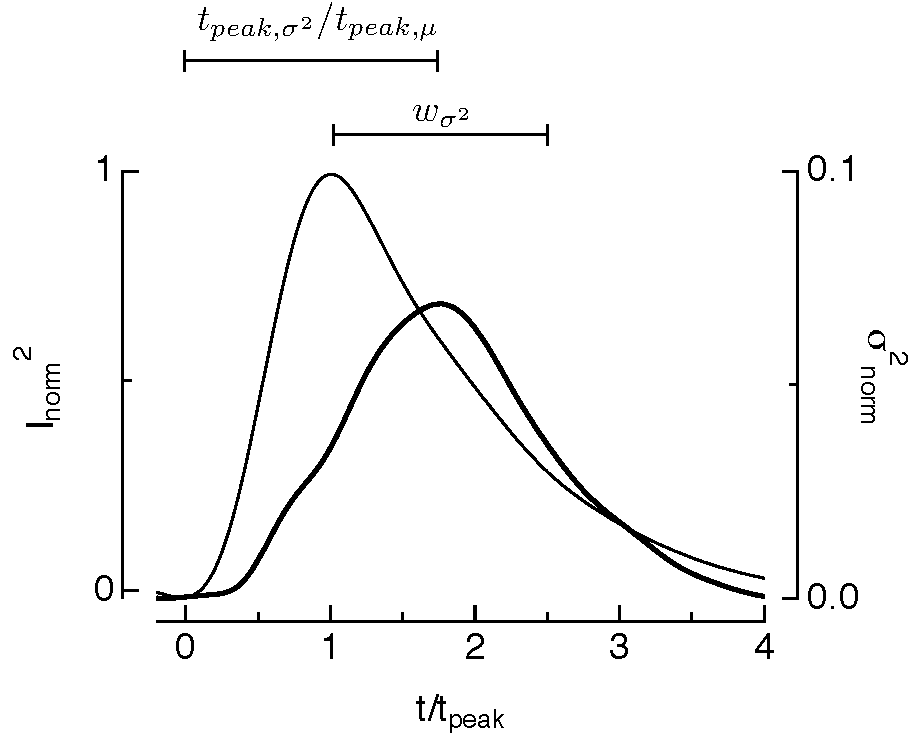
\includegraphics[width=4in]{params.pdf}
\caption{Parameters used in likelihood analysis.}  
\label{fig:likelihood-params}
\end{center}
\end{figure}


We evaluated the likelihood of a given model based on comparison of these parameters with experiment.  To do this, we measured the mean and SEM of the parameters across recorded rods, assumed the distribution of parameters was a multi-variant Gaussian, and then determined how far (in units of SEM) the model was from the mean of the experimental points for each parameter.  Converting these distances to probabilities and multiplying across parameters provided an estimate of the likelihood of a given model.  This provided a direct measure of how well a given model captured key features of the experimental responses.  

%Test is then to see if properties of response variability are well captured.  Use this approach in particular to compare transgenic manipulations expected to produce changes in $F$ but not $R$ (\GCAPHET, \GCAPKO), or possibly changes in $R$ but not $F$ (\ArrHET, \RKHET; these are complicated because we do not know how they change $R$).

\subsection{Spatio-temporal diffusion model}

In addition to two empirical models for compression above, investigate more mechanistically based spatio-temporal diffusion model as studied by Bisegna et al.  It may map onto first case above.  In any case this is important since they have suggested that local depletion of cGMP could cause reduced sensitivity to variability in PDE activity and hence contribute to reproducibility.


%%%%%%%%%%%%%%%%%%%%%%%%%%%%%%%%%%%%%%%%%
 
\section{Results}

Our aim is to use the measured single photon responses in rods from wild-type and genetically-altered mice to constrain models for rhodopsin inactivation and transducin activation.  We start with several general theoretical considerations, then test linearity of the transduction process, and finally evaluate stochastic models for rhodopsin and transducin activity using measured responses.  
 
\subsection{Two theoretical predictions}

A linear transduction process, regardless of its kinetic properties, does not change the coefficient of variation of the single photon response area.  Thus, if rhodopsin is the only stochastic component in the transduction process, and the relationship between rhodopsin's activity and the membrane current is linear, the coefficient of variation of the current area is identical to the coefficient of variation of rhodopsin's integrated or cumulative activity.  Intuitively, this equality originates because the relation between the area of a given rhodopsin trajectory and the current is given by the area of the linear transduction filter --- i.e. a single scalar number.  The area of every rhodopsin trajectory gets multiplied by the same scalar to produce the area of the current response, but such a scaling of responses does not alter the coefficient of variation since it effects the mean and standard deviation of the responses equally.  

The lack of an effect of linear filtering on \CVArea means that the measured \CVArea provides an upper bound on variability in rhodopsin's cumulative activity.   This is an upper bound because it associates all of the response variability with rhodopsin, while some variability likely originates in post-rhodopsin components of the transduction process (particularly transducin, see below).  Thus while changes in the kinetics of rhodopsin inactivation relative to the transduction process can alter which temporal components of the response vary, they do not change the total response variability (Figure~\ref{fig:linearity-and-variability}).  Thus in the context of multi-step shutoff models for rhodopsin inactivation, the measured \CVArea of 0.3 to 0.35 requires a minimum of 8 to 11 (i.e. CV$_{area} = 1/\sqrt{N}$) steps. 

\begin{figure}[h]
\begin{center}
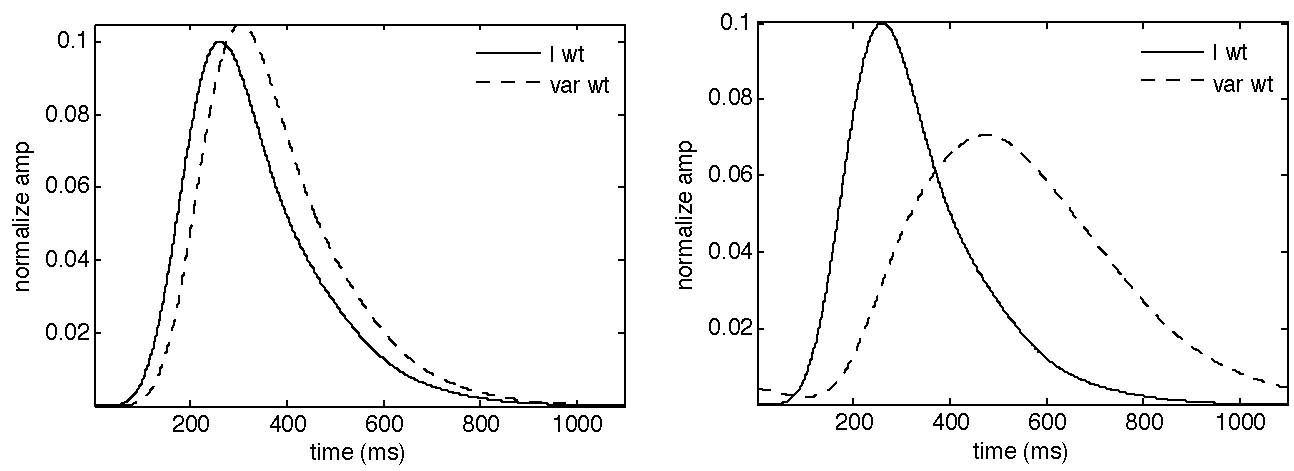
\includegraphics[width=5in]{linearity-and-variability.pdf}
\caption{Predicted squared mean and time-dependent variance for rapid (left) and slow (right) rhodopsin inactivation.  Models assume that the transduction process is linear and that response variability is produced entirely by rhodopsin.  Both models identically replicate the measured wild-type mean single photon response, and the \CVArea of both models is 0.35 --- i.e. $1/\sqrt{N}$ with $N=8$ shutoff steps.}  
\label{fig:linearity-and-variability}
\end{center}
\end{figure}

The discussion above emphasizes the contribution to response variability from trial-to-trial variations in rhodopsin activity.  Response variations due to the finite number of activated transducin (or PDE) molecules pose another potential source of response variability.  The number of transducin activations during a single step in rhodopsin activity is expected to follow a geometric distribution (see Methods).  Assuming linearity of the transduction process, the measured \CVArea then also provides a lower bound on the number of activated transducins.  In particular, if we assume that rhodopsin makes no contribution to response variability, and that transducin activation is on average spread uniformly across rhodopsin shutoff steps, \CVArea $ = \sqrt{2/n_T}$, there $n_T$ is the mean total number of transducin activations.  Thus the measured \CVArea of 0.3 to 0.35 requires at least 16 to 22 transducin activations.  
   
More generally, with a linear transduction process, $m$ steps in rhodopsin inactivation and an average of $N$ total activated transducin molecules, \CVArea~is
\begin{equation}
{\rm CV}_{area}  = \sqrt{{1 \over N} + {2 \over n_T}}.
\end{equation}
Figure~\ref{fig:theory-limits} plots the dependence of \CVArea on $n_T$ for several choices of $N$.  The dashed line plots the measured \CVArea --- i.e. allowable values of $n_T$ and $N$, assuming linearity of the transduction process, fall below the dashed line.  

\begin{figure}[h]
\begin{center}
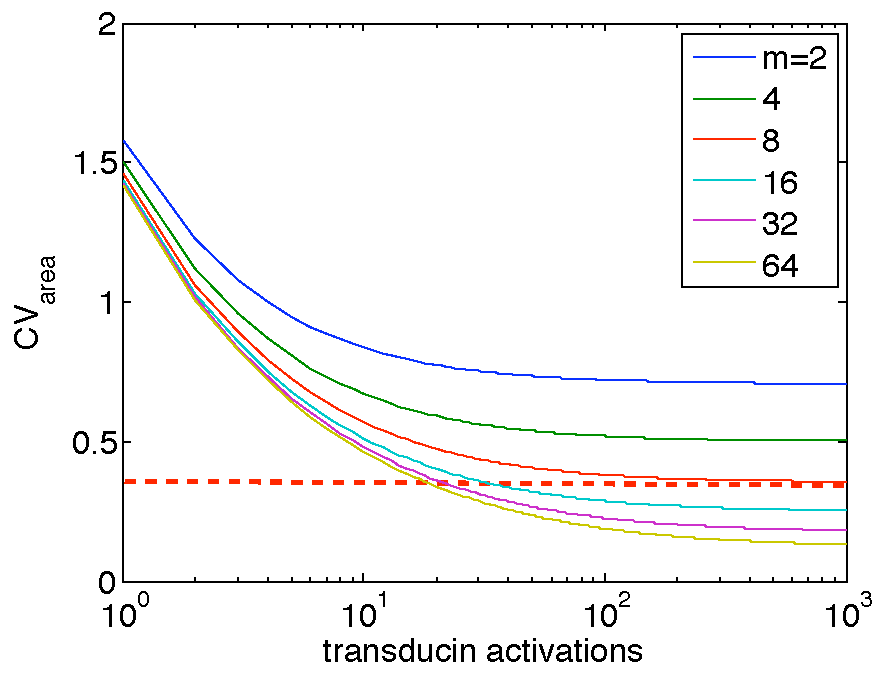
\includegraphics[width=3in]{theory-limits.pdf}
\caption{Predicted \CVArea as number of steps in rhodopsin shutoff and number of transducin activations are varied.  Dashed red limit plots measured \CVArea.}  
\label{fig:theory-limits}
\end{center}
\end{figure}

Although variability introduced by rhodopsin and transducin can have similar effects on \CVArea, they have different effects on the shape of the time-dependent variance of the responses.  One of the experimental signatures of single photon response variability is the late time-to-peak of the variance --- i.e. most of the variance of the responses occurs during response recovery rather then initial rise.  Models in which variability is dominated by transducin activation fail to capture this late variance, unlike those in which rhodopsin inactivation is both dominant and slow (Figure~\ref{fig:TvsRh}).  The inability of variability associated with transducin activation to capture the late peak of the variance observed experimentally remains across a wide range of relative durations of rhodopsin and transducin activity.  It originates because variability associated with transducin tracks the mean responses.  

\begin{figure}[h]
\begin{center}
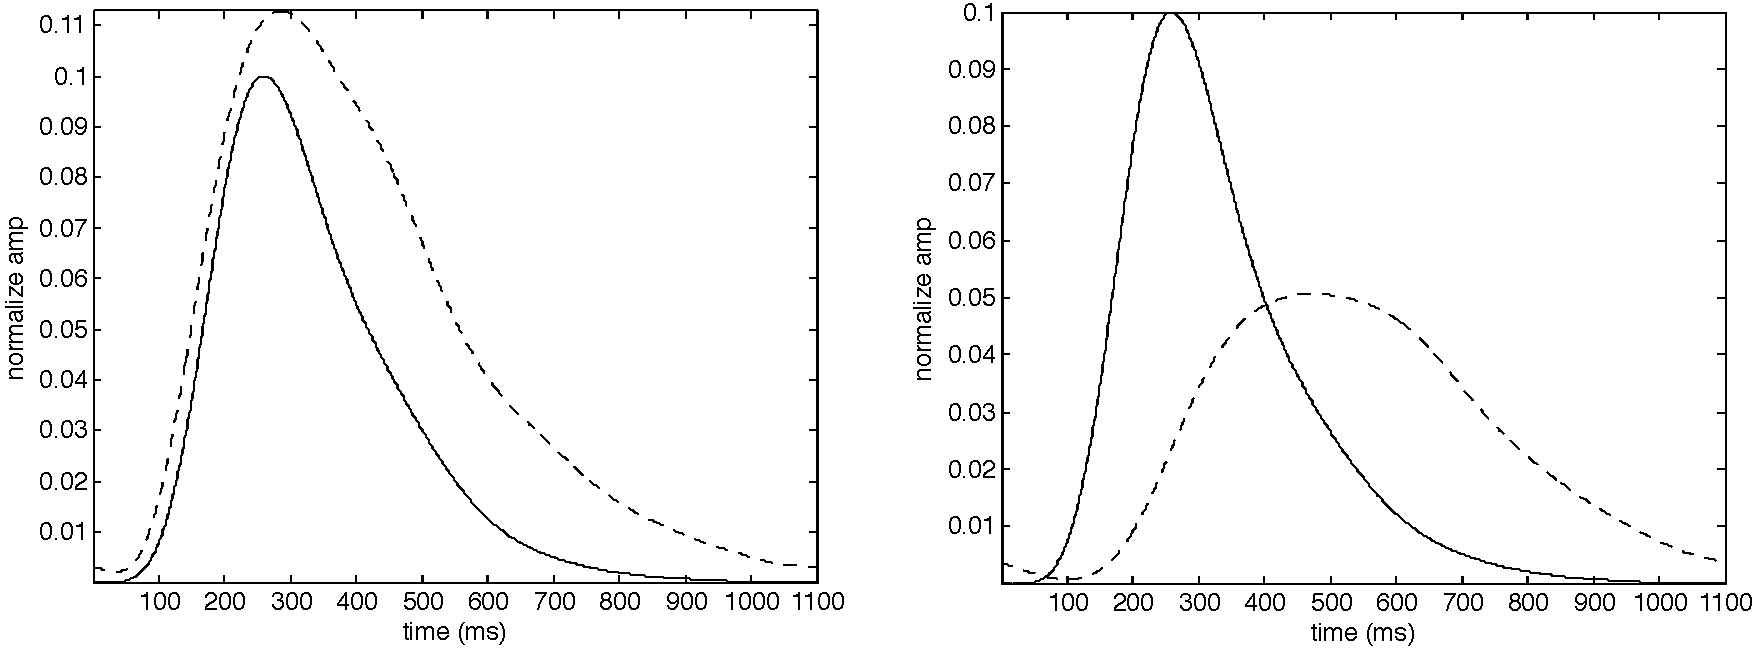
\includegraphics[width=5in]{TvsRh.pdf}
\caption{Time-dependent variance and square of mean response for models with stochastic transducin activation (left) and stochastic rhodopsin inactivation (right).}  
\label{fig:TvsRh}
\end{center}
\end{figure}

%%%%%%%%%%%%%%%%%%%%%%%%%%%%%%%%%%%%%%%%%

\subsection{Linearity of the transduction process}

As described above, both rhodopsin and transducin activities are highly constrained by the measured low variability of the single photon response provided the transduction process is linear.  Thus we sought to test linearity of the cascade directly.  Linearity could fail in two broad ways: (1) nonlinear interactions of the disc-associated reactions --- e.g. depletion of available transducin or PDE; (2) nonlinearities associated with the post-disc reactions --- e.g. depletion of cGMP or channels.  This separation is important for interpretation of experiments aimed at testing linearity.

Past work supports linearity of the transduction process.  First, Burns et al. found that a differences in both single photon responses and continuous noise of wild-type and \GCAPKO rods could be accounted for by a single linear change in transduction.  Thus a linear filter that accounted for differences between the estimated single photon response of wild-type and \GCAPKO rods also could account for differences in continuous noise.  Continuous noise involves much smaller local changes in the activity of the transduction cascade than the single photon response, and hence saturating nonlinearities in the cascade would be expected to effect the single photon response more than the noise.  Thus their results argue that the calcium feedback to the cyclase operates in an effectively linear manner during the single photon response.  This experiment does not directly test linearity of the disc-associated reactions.  

Second, Field and Rieke found that responses to two nearby photons added linearly or near linearly in primate and guinea pig rods.  Flashes delivered through a slit $\sim$1-2 $\mu$m in width summed linearly up to 5-6 Rh*.  This region contains 50-100 discs, so the experiment does not test for nonlinearities in the disc-associated reactions.  The relationship between this experiment and depletion of cGMP at active PDE depends on whether the depletion of cGMP produced by activity on one disc extends reduces the cGMP level at the PDE in surrounding discs. 

\begin{figure}[h]
\begin{center}
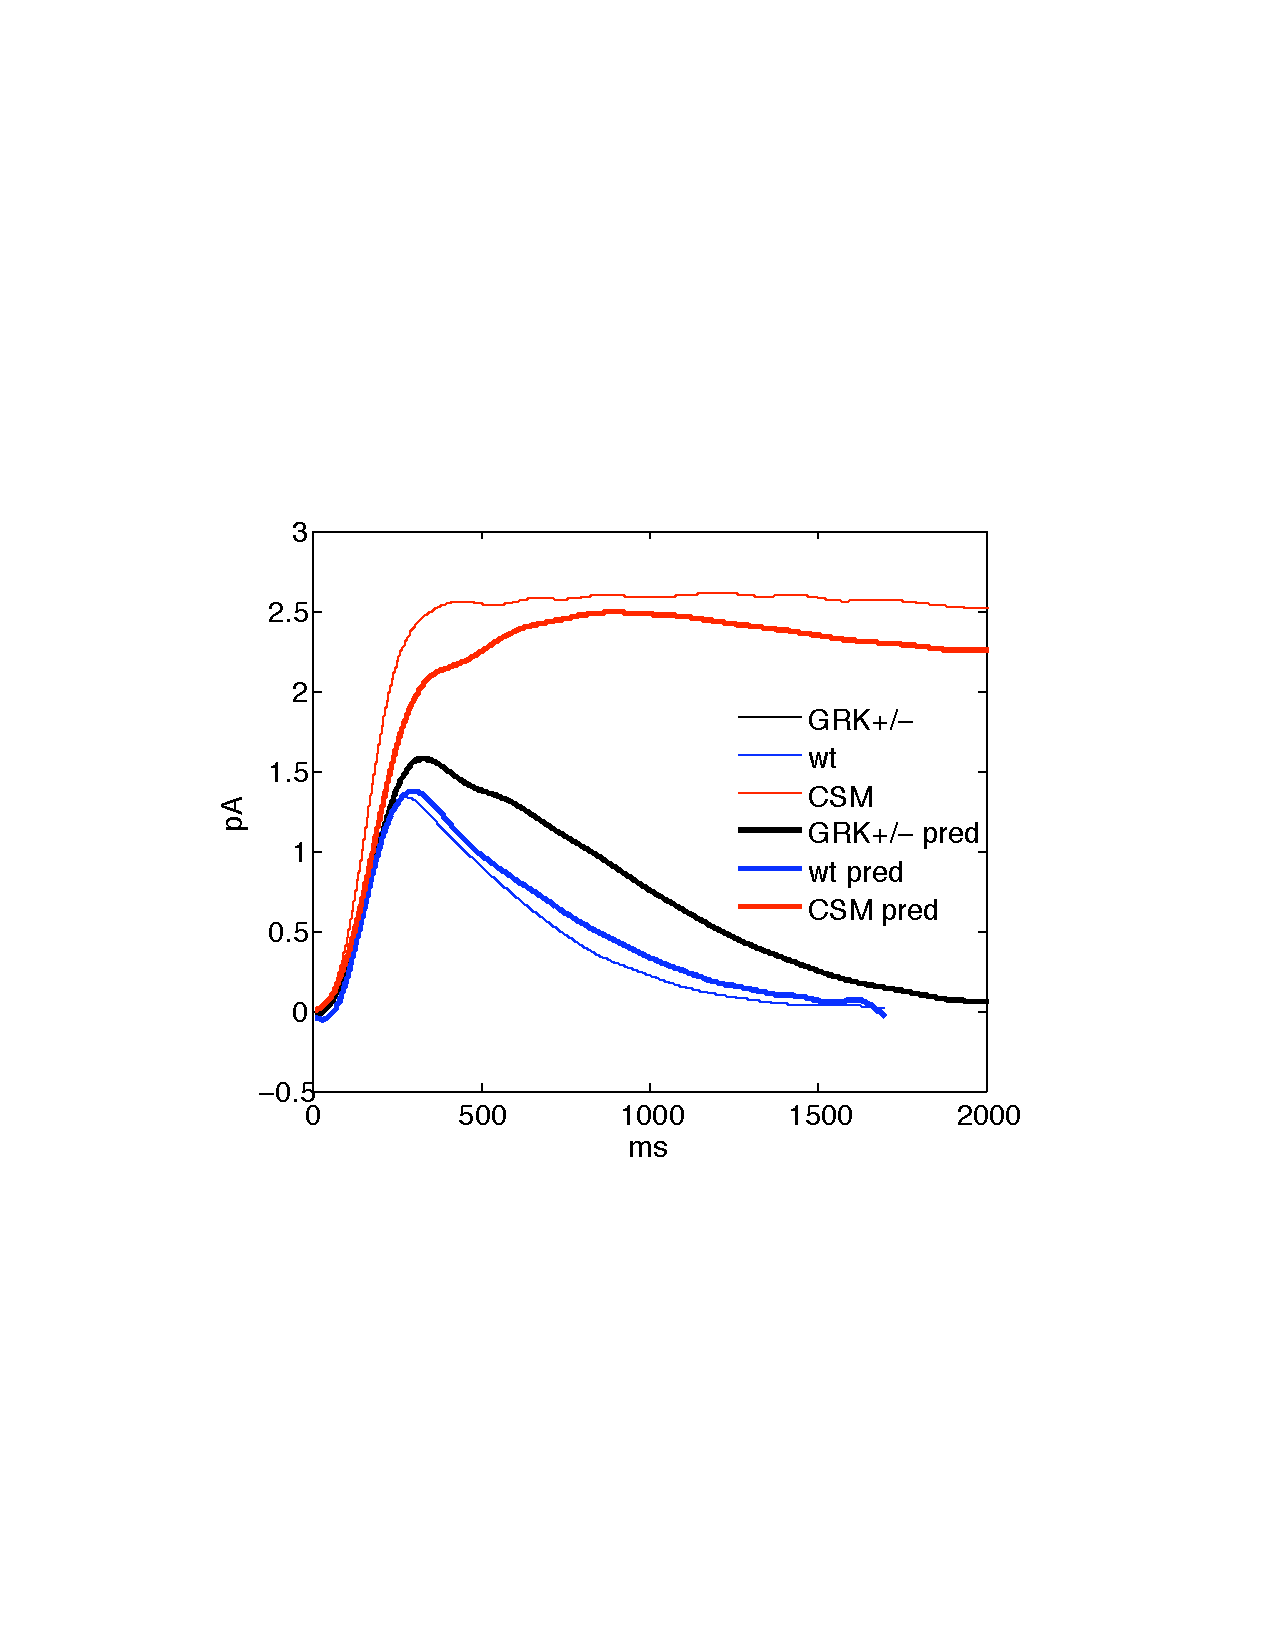
\includegraphics[width=3in]{linearity.pdf}
\caption{Measured and predicted single photon responses assuming common linear transduction cascade, constrained by Pepperberg time constant and single photon response measured in wt mice (smallest response).  $R^*(t)$ assumed to decay with time constant of 370 ms for wt, 640 ms for GRK$^{+/-}$.  Transduction filter fit to \RKHET response.}  
\label{fig:linear-predict}
\end{center}
\end{figure}

\begin{figure}[h]
\begin{center}
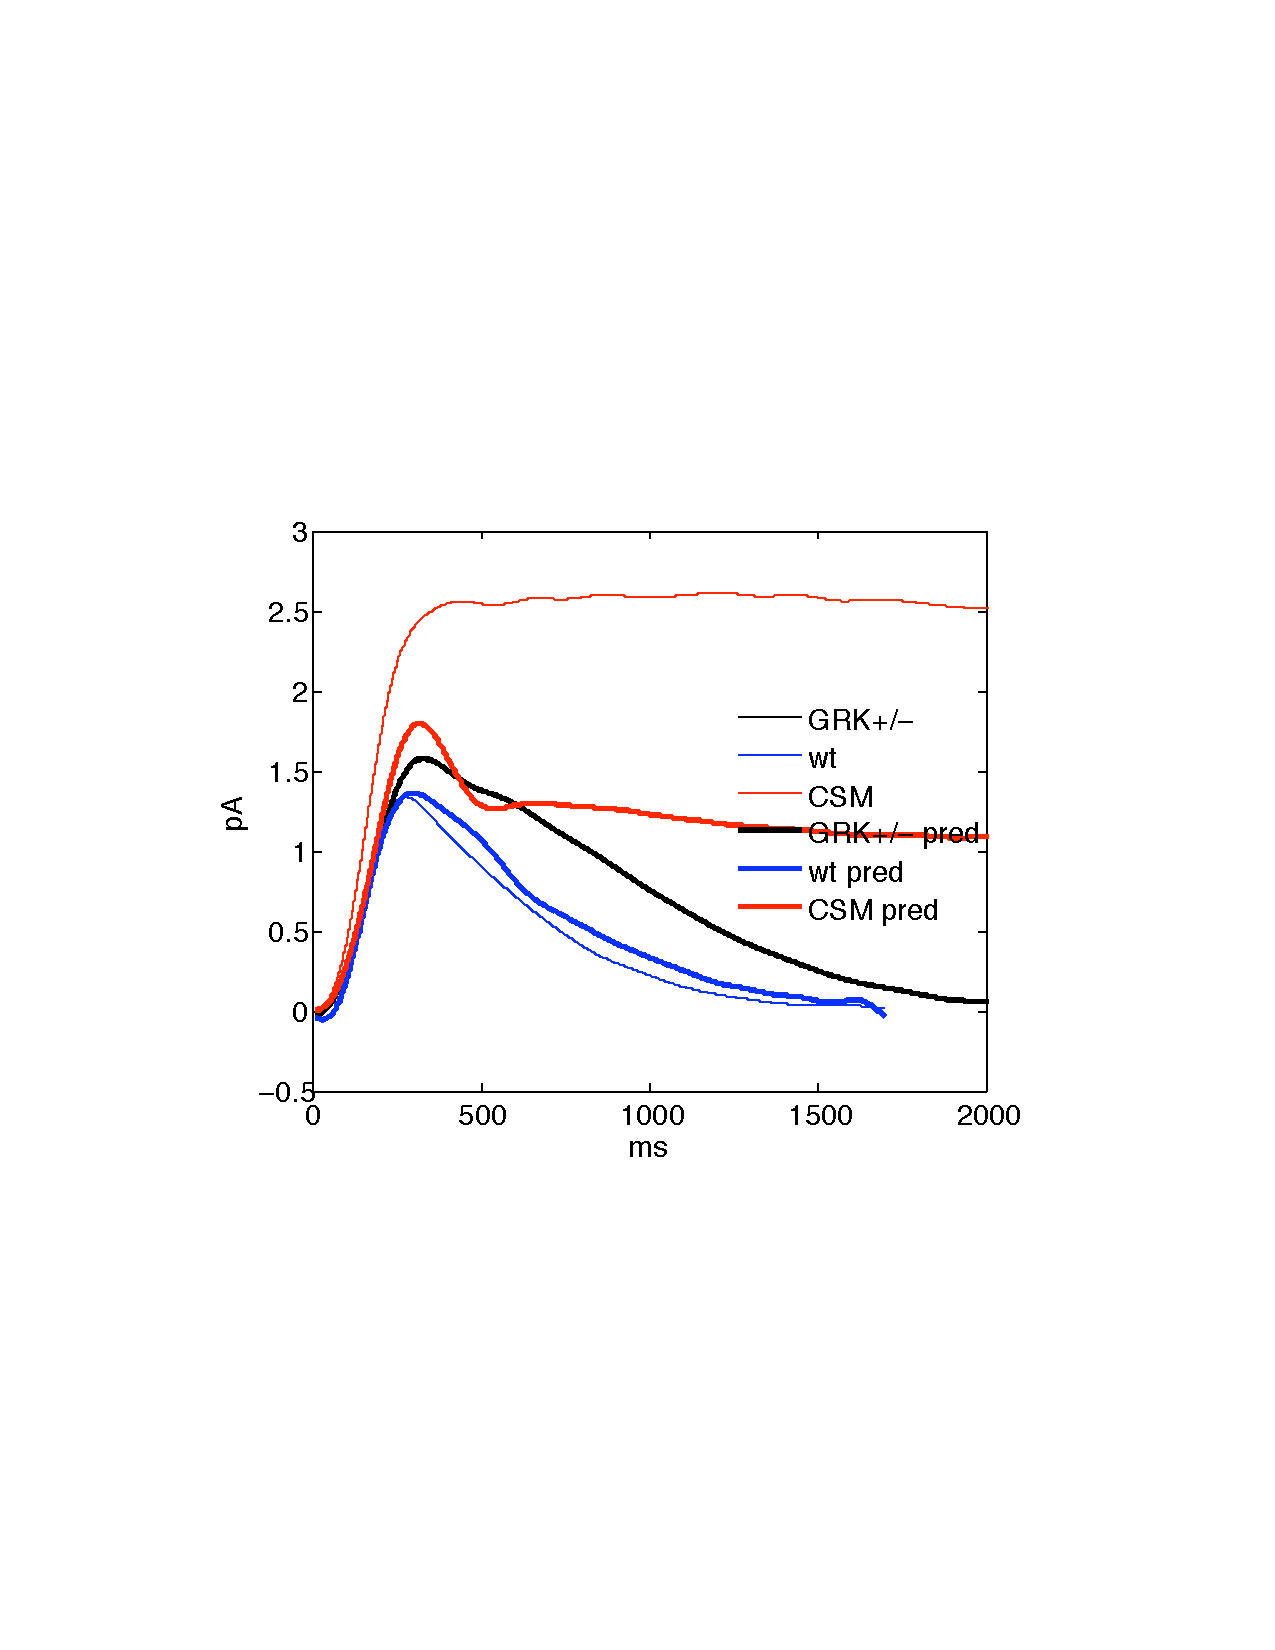
\includegraphics[width=3in]{nonlinearity.pdf}
\caption{Measured and predicted single photon responses including thresholded PDE activity.  PDE decay time constant 200 ms, thresholding nonlinearity set to peak of \RKHET~PDE activity.  Other parameters as above.}
\label{fig:nonlinear-predict}
\end{center}
\end{figure}

To provide an additional and more complete test of linearity, particularly of the disc-associated reactions, we compared quantitatively responses of wild-type and genetically-altered mouse rods.  The comparison leading to the clearest interpretation was between rods with a reduction in rhodopsin kinase concentration (\RKHET) and rods with no phosphorylation sites (CSM).  As observed previously, responses produced by rhodopsin without phosphorylation sites are larger than those with less drastic alterations in rhodopsin inactivation and show little recovery during the initial 1-2 sec following photon absorption (Figure~\ref{fig:linear-predict}).  We sought to explain this difference quantitatively and in doing so test linearity of the transduction process.  The essence of the argument is that the greater rhodopsin activity in the CSM rods should exacerbate the effects of any saturating nonlinearities in transduction.  By testing manipulations of rhodopsin activity rather than downstream components of the cascade, we test for both disc-associated and post-disc nonlinearities.

We calculated the linear transduction filter $F$ from the \RKHET~responses following Eq.~\ref{eq:linear-trans}.  This requires making an assumption about the average time course of rhodopsin activity $R(t)$.  The dominant time constant for the decay of light-activated PDE activity is prolonged in \RKHET~rods compared to wild-type rods under our recording conditions; this result indicates that the dominant time constant reflects the time course of rhodopsin inactivation.  Hence we assume that $R(t)$ is exponential with a 640 ms time constant; we relax this constraint on the shape of $R(t)$ below.  We use $R(t)$ and the measured single photon response to determine the linear transduction filter $F$.  We then used this filter to predict the responses produced by rhodopsin lacking phosphorylation sites altogether (CSM rods).  Based on the initial lack of recovery of the single photon response, we assume that $R(t)$ is a step function, with peak amplitude equal to that of rhodopsin activity in \RKHET~rods.  Thus the predicted $I(t)$ in this case is the integral of $F$ (i.e. $F$ convolved with a step function).  Nonlinearities that could contribute to reproducibility should reduce the gain of the coupling of rhodopsin and the membrane current as the response progresses; the effect of nonlinearities should be exacerbated for the longer-lasting rhodopsin activity in the CSM rods, causing the measured response to fall short of the linear prediction.  

Fig.~\ref{fig:linear-predict} compares predicted and measured responses.  The predicted responses assuming a linear transduction process are, if anything, slightly smaller than those measured.  This difference is opposite the expectation for compressive nonlinearities in transduction.  As a control for alterations in the transduction cascade that could cause unexpected changes in the response, we repeated these experiments in \RKHET rods expressing both normal rhodopsin and rhodopsin with one remaining phosphorylation site; the CSM line was no longer available, but responses produced by rhodopsin with a single phosphorylation site were nearly identical.  More re results here.

The ability of a common linear filter to account for both \RKHET and CSM responses leaves open two possibilities: either the transduction process is close to linear, or it is so nonlinear that the degree of nonlinearity does not change between \RKHET and CSM rods --- i.e. the \RKHET responses are already strongly saturated, but the period of such saturation is prolonged in CSM rods, leading to a larger response.  In the later case, the resemblance of the linear prediction to the measured response in Fig.~\ref{fig:linear-predict} would be fortuitous.  To test model 2 --- i.e. a strong saturation that applies to all responses ---  we extended the analysis to include saturation of the PDE activity.  We assume that the PDE activity is given by convolving $R(t)$ with an exponential to represent the transducin inactivation time constant, and apply a thresholding nonlinearity to the resulting $P(t)$ such that any values of $P(t)$ exceeding the threshold are set to the threshold value.  We then compute the linear filter between $P$ and $I$, assume that this filter and the threshold are fixed, and predict changes in response for \RKHET~and CSM rods.  

Figure \ref{fig:nonlinear-predict} shows results of this analysis, assuming a transducin decay time constant of 300 ms and a threshold set to the peak of the PDE activity for the \RKHET response.  This value for the threshold does not impact \RKHET or wild-type responses, and hence would not be effective in reducing their variability.  Lower thresholds, i.e. those that could contribute to reproducibility, further reduce the predicted CSM response.  A threshold applied to the current itself (e.g. depletion of channels) would simply scale the entire predicted response down.  Thus the \RKHET and CSM responses are inconsistent with a strong thresholding nonlinearity operating either on the PDE activity or cGMP channels.

%A possible intuitive explanation for the failure of a nonlinear model is as follows.  The filter coupling $P^*$ to $I$ has relatively brief time constants - and hence the kinetics of $I$ do not differ dramatically from $P^*$ (at least under the experimental conditions of our measurements, with numbers above).  In this case, the cGMP concentration (and membrane current) do not lag far behind the PDE activity.  Further, with comparable time constant for rhodopsin and PDE decay, the PDE activities in wt, RK$^{+/-}$ and CSM rods all rise along a similar trajectory.  Thus they should all reach a threshold at roughly similar times.  Together these mean that the predicted CSM response will approximately rise along the same trajectory as the wt response, and then run flat at the peak amplitude of the wt response.  Substantial alterations in parameters change this picture quite a bit --- but they have to be pretty dramatic changes (e.g. taking R* inactivation time constant for \RKHET rods to 100 ms).  With such changes the predicted CSM response can be much larger than wt, but the large response comes about with a slow rising phase (initially along wt trajectory, than slowing before reaching a constant level around 700 ms). 

\bigskip
\noindent
NOTES:

\bi

\i{should wt data be included in above?  Requires assuming something about rhodopsin time constant - or that could be backed out of data by deconvolving filter from measured response.}

\i{do analysis and add using different $R(t)$ trajectories corresponding to gradual or abrupt shutoff.}

\i{try to replicate results with spatio-temporal diffusion model?}

\i{analyze \GCAPKO single photon response and noise re linearity, add to this section.}

\i{rgs9 overexpressors could test for saturation by decreasing transducin activity - would expect increase in CV if compression at PDE}

\ei

%%%%%%%%%%%%%%%%%%%%%%%%%%%%%%%%%%%%%%%%%

\subsection{Constraints on stochastic models for rhodopsin inactivation}

How many shutoff steps contribute to rhodopsin inactivation?  What is the effect of each step on rhodopsin's catalytic activity?  What is the duration of rhodopsin's catalytic activity?  We evaluated models for the single photon response that specifically instantiated these parameters.  We generated an ensemble of single photon responses for each combination of model parameters and compared modeled and experimental responses.  In particular, we asked how well the model captured the total response variability (\CVArea), the time-to-peak of the variance relative to the mean response (\tpeakratio), and the width of the variance ($w_{\sigma^2}$) (see Fig. xx).  We evaluated the likelihood of each model using experimental values of the mean and SEM of these parameters (see Methods). 

\begin{figure}[h]
\begin{center}
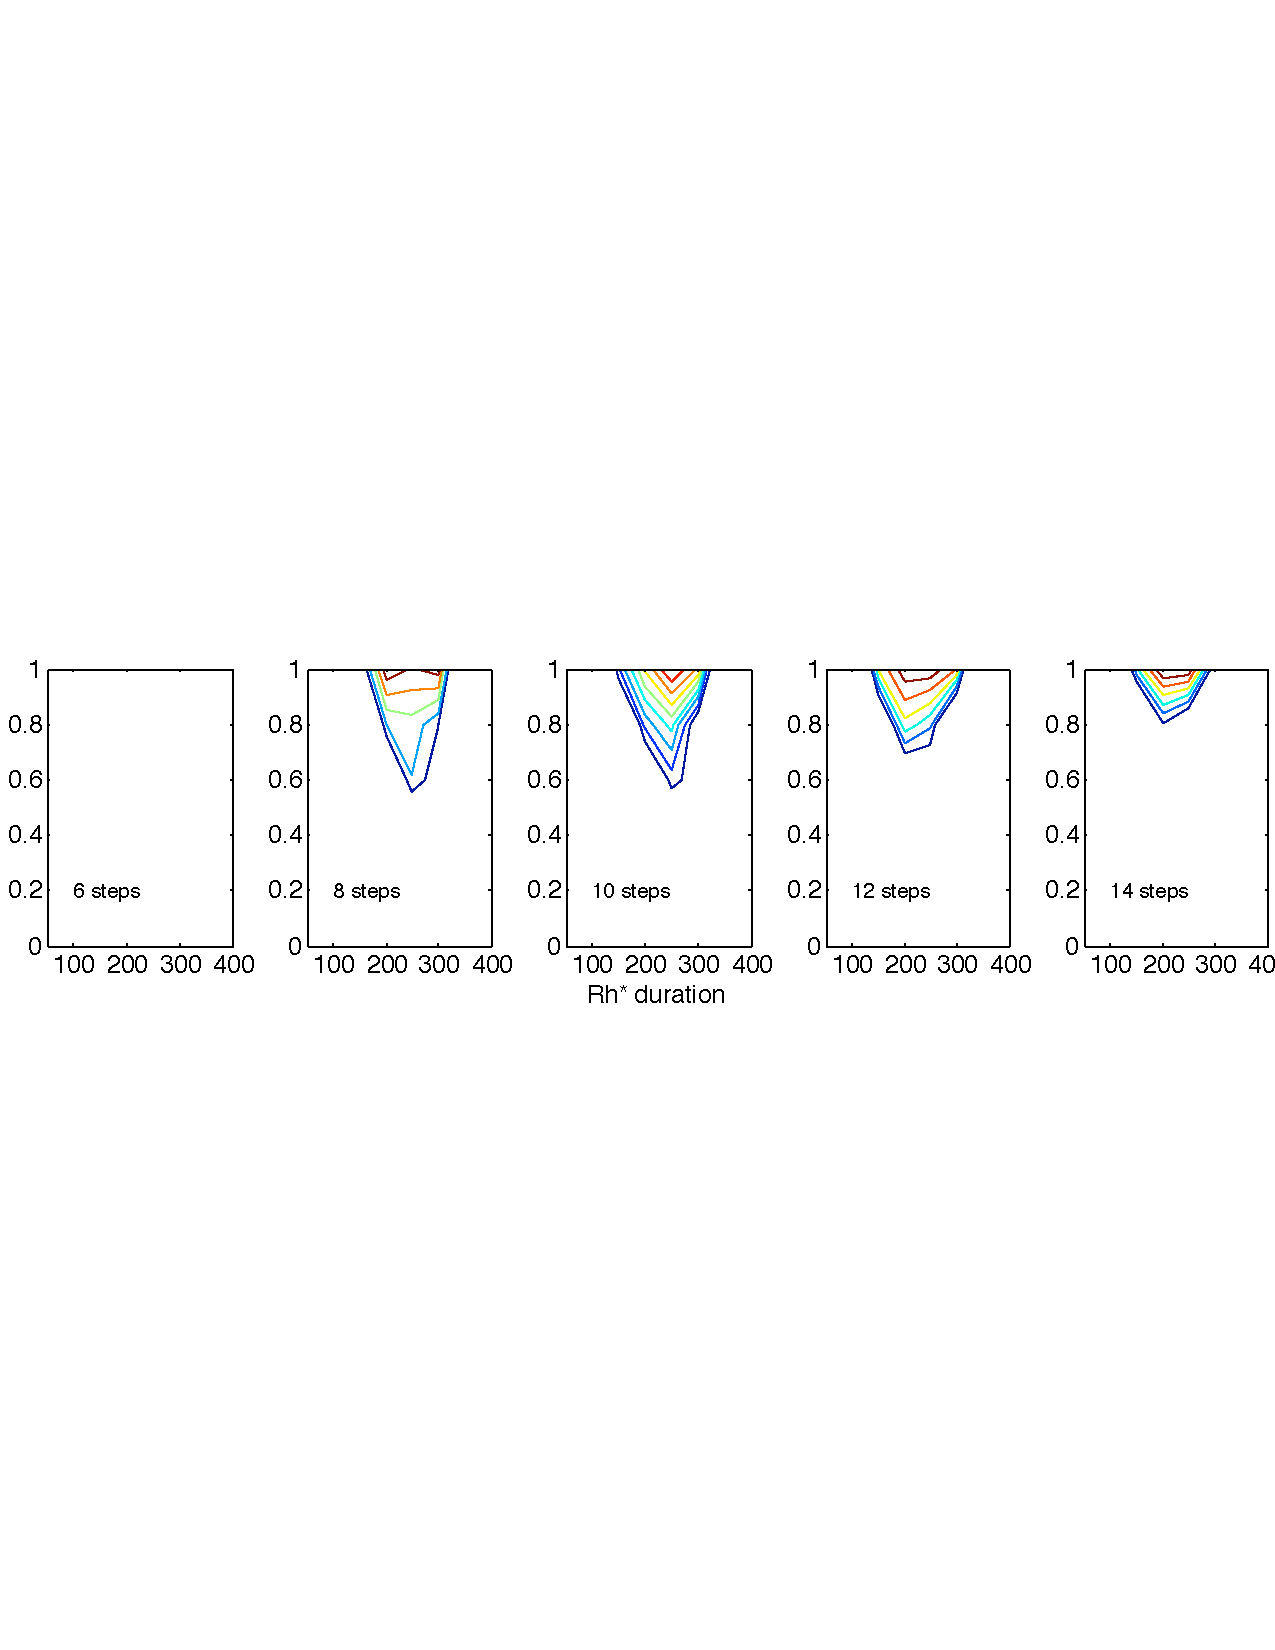
\includegraphics[width=6in]{likelihood_wt.pdf}
\caption{Likelihood analysis of linear models. Y-axis is rhodopsin decay factor.}
\label{fig:likelihood}
\end{center}
\end{figure}

\begin{figure}[h]
\begin{center}
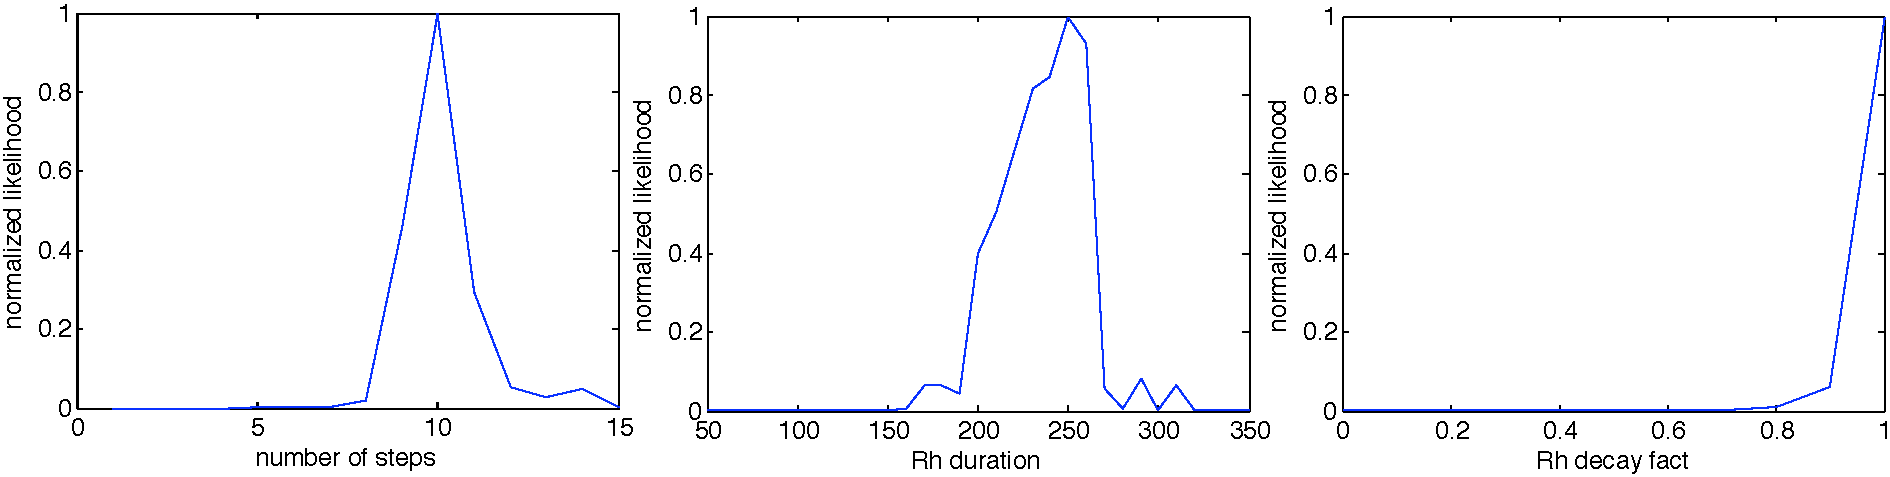
\includegraphics[width=6in]{likelihoodcuts.pdf}
\caption{Likelihood analysis of linear models.  Parameters other than that varied were held fixed at their peak values.}
\label{fig:likelihoodcuts}
\end{center}
\end{figure}

We start by considering models with linear transduction cascades and deterministic transducin activation.  We varied the number of steps in rhodopsin inactivation ($N$), the duration of rhodopsin's activity ($\tau_{Rh}$), and the decrease in activity for each step ($\alpha$).  Figure~\ref{fig:likelihood} shows likelihood calculated for a range of values for $N$, $\tau_{Rh}$ and $\alpha$.  Each contour represents a 3-fold change in likelihood.  The likelihood has a strong dependence on these parameters, reaching a peak for 10 inactivation steps, a time constant of 240 ms and an equal decay of activity produced by each step ($\alpha = 1$).  These parameters of rhodopsin inactivation had relatively independent effects on likelihood.  Figure~\ref{fig:likelihoodcuts} shows the dependence on each parameter separately; the parameters that were not varied were fixed at their optimal values.  The likelihood decreased more than 10-fold for $>$ 20\% changes in any of these parameters away from the peak values.

Figure~\ref{fig:GCAPlikelihood} shows the same analysis applied to \GCAPKO responses.  GCAP mediates calcium feedback regulation of the rate of cGMP synthesis; the GCAP-mediated acceleration in synthesis is an important component of timely response recovery.  Thus deletion of GCAP is expected to change the shape of the single photon response.  If the role of GCAP is restricted to altering the filtering properties of the transduction cascade rather than altering response variability, we would expect a common stochastic model for rhodopsin inactivation to account for responses in both cases.  Indeed, the likelihood evaluated from \GCAPKO responses peaked for very similar parameters at wild-type responses: 10 steps, 225 ms rhodopsin duration and equal decay of activity for each step.  The likelihood depended strongly on the number of steps and rhodopsin duration, but was relatively insensitive to how much rhodopsin decayed with each inactivation step. 

An intuitive explanation for the dependence of likelihood on various parameters follows.  For linear models, \CVArea is controlled entirely by the number of inactivation steps and hence directly constrains this parameter.  \tpeakratio depends primarily on the duration of rhodopsin's activity relative to the kinetics of the transduction cascade filter (Figure~\ref{fig:linearity-and-variability}), with a weak dependence on the number of steps.  Finally the width of the variance is primarily determined by how much activity declines following each step; with little decline following each step, the variability all occurs in a narrow window following the final decay step, while with a distribution of decay across steps variability is more spread out over time.

\begin{figure}[h]
\begin{center}
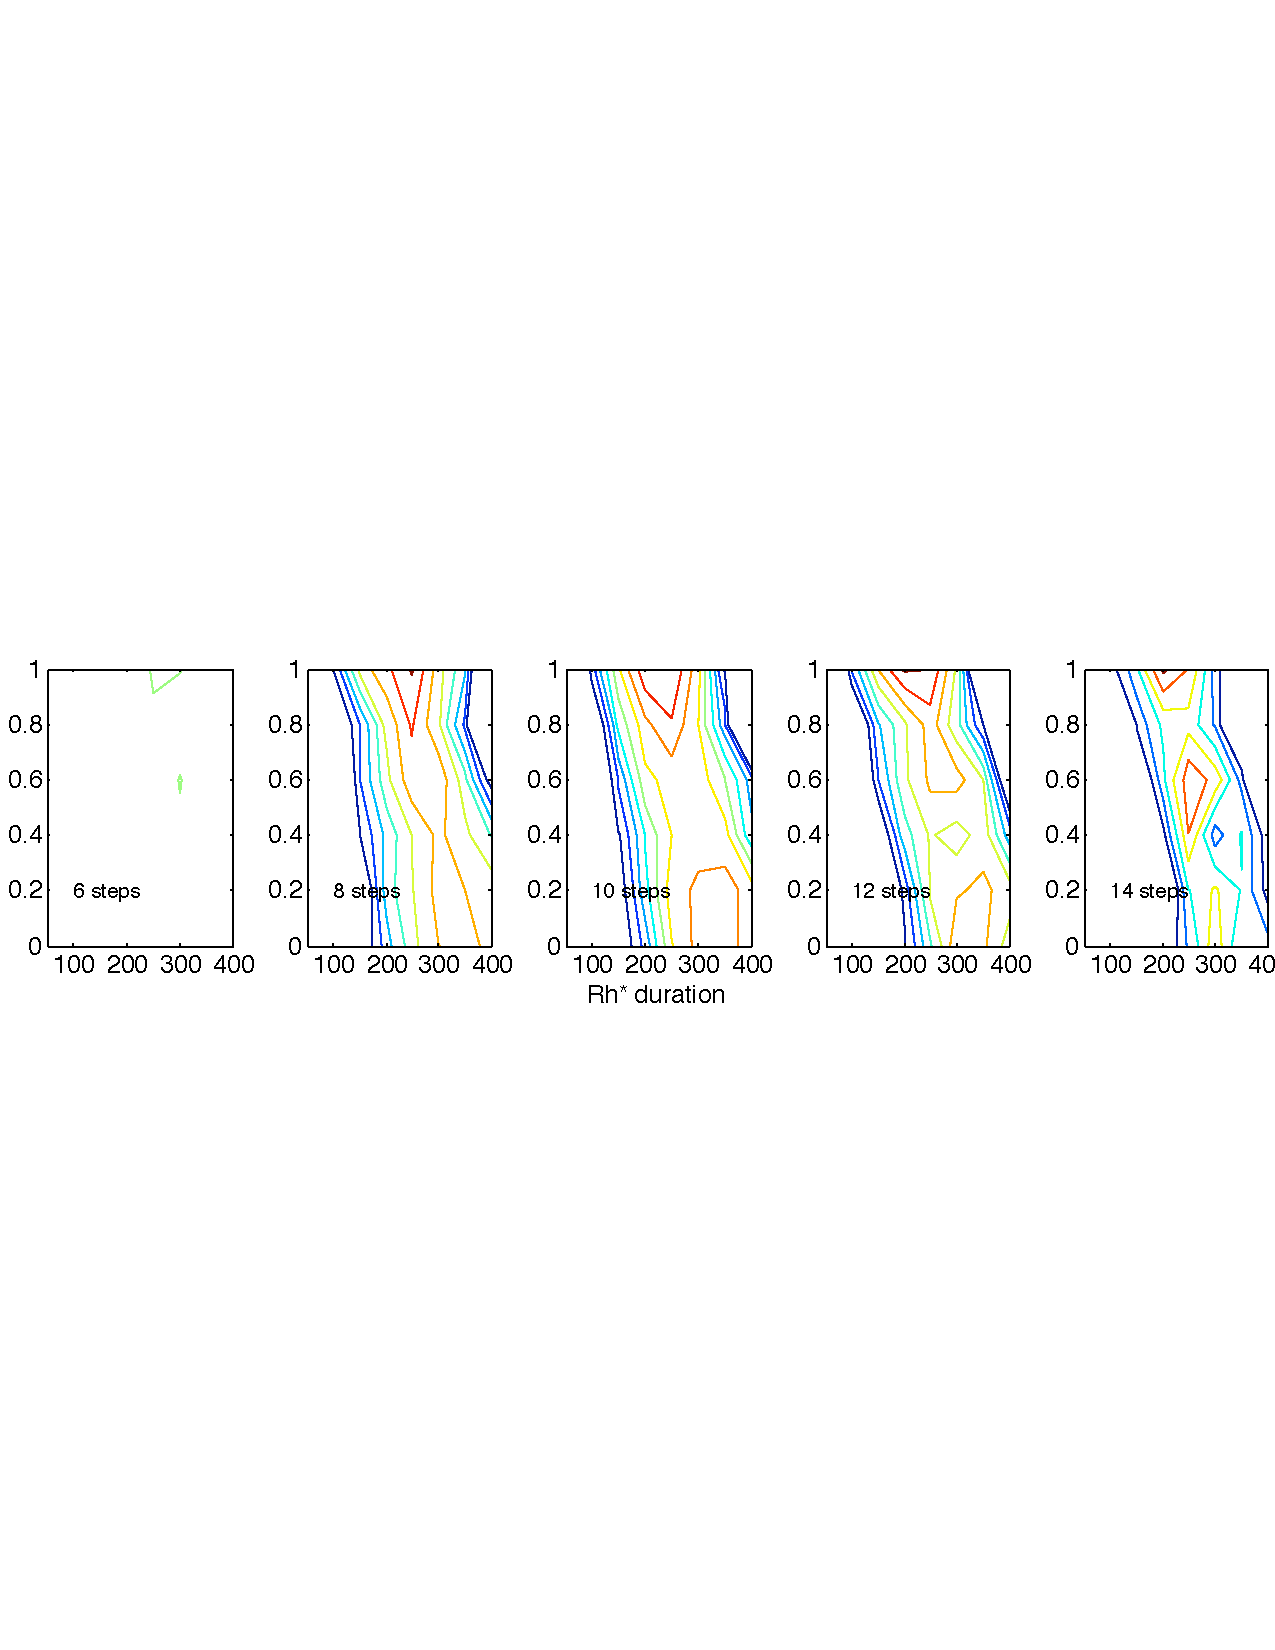
\includegraphics[width=6in]{GCAPlikelihood.pdf}
\caption{Likelihood analysis of linear models, \GCAPKO responses.}
\label{fig:GCAPlikelihood}
\end{center}
\end{figure}

\begin{figure}[h]
\begin{center}
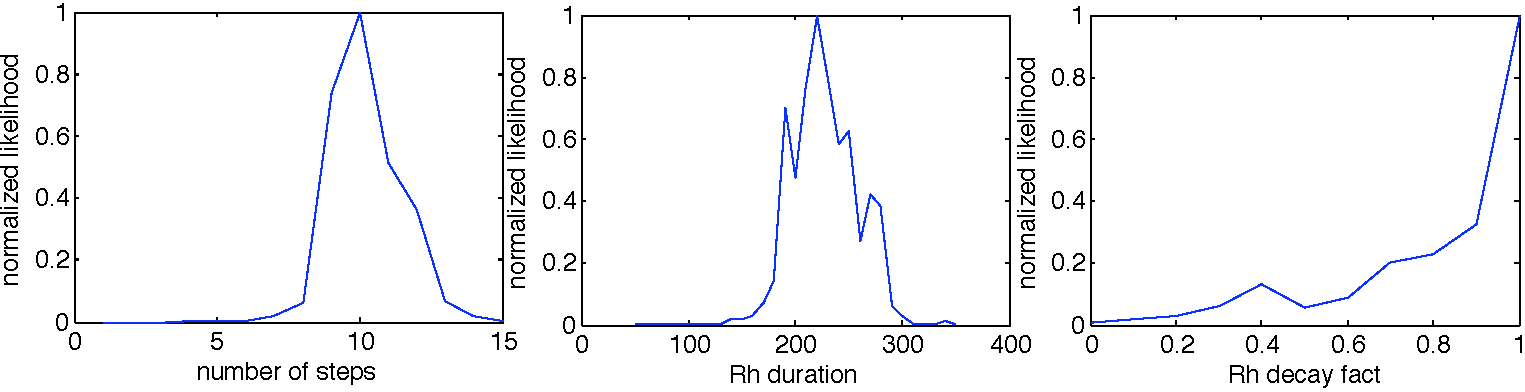
\includegraphics[width=6in]{GCAPlikelihoodcuts.pdf}
\caption{Likelihood analysis of linear models, \GCAPKO responses.}
\label{fig:GCAPlikelihoodcuts}
\end{center}
\end{figure}

We also evaluated models that included a compressive nonlinearity limiting the peak transducin activity.  In this case we varied the rhodopsin inactivation time constant, the number of shutoff steps and the extent of compression.  We held the decay of rhodopsin activity for each inactivation step fixed at its optimal value of 1 (equal decay across steps) as determined above.  Good fits to the experimental data could be retained with transducin compression by decreasing the number of inactivation steps and increasing the rhodopsin duration (Figure~\ref{fig:TrCompression}).  For example, similar likelihoods could be achieved with no compression, a 240 ms rhodopsin duration and 10 inactivation steps, or with compression, a 360 ms rhodopsin duration and 4 inactivation steps.  The longer rhodopsin duration is required because adding compression and decreasing the number of steps decreases the late variance in the response; hence obtaining good fits requires compensating by increasing the duration of rhodopsin's activity, which shifts the time-dependent variance to later times.  Increasing the duration of transducin's activity is not effective in creating a late peak in the time-dependent variance (see Figures~\ref{fig:linearity and variability} and \ref{fig:TvsRh}).  

\begin{figure}[h]
\begin{center}
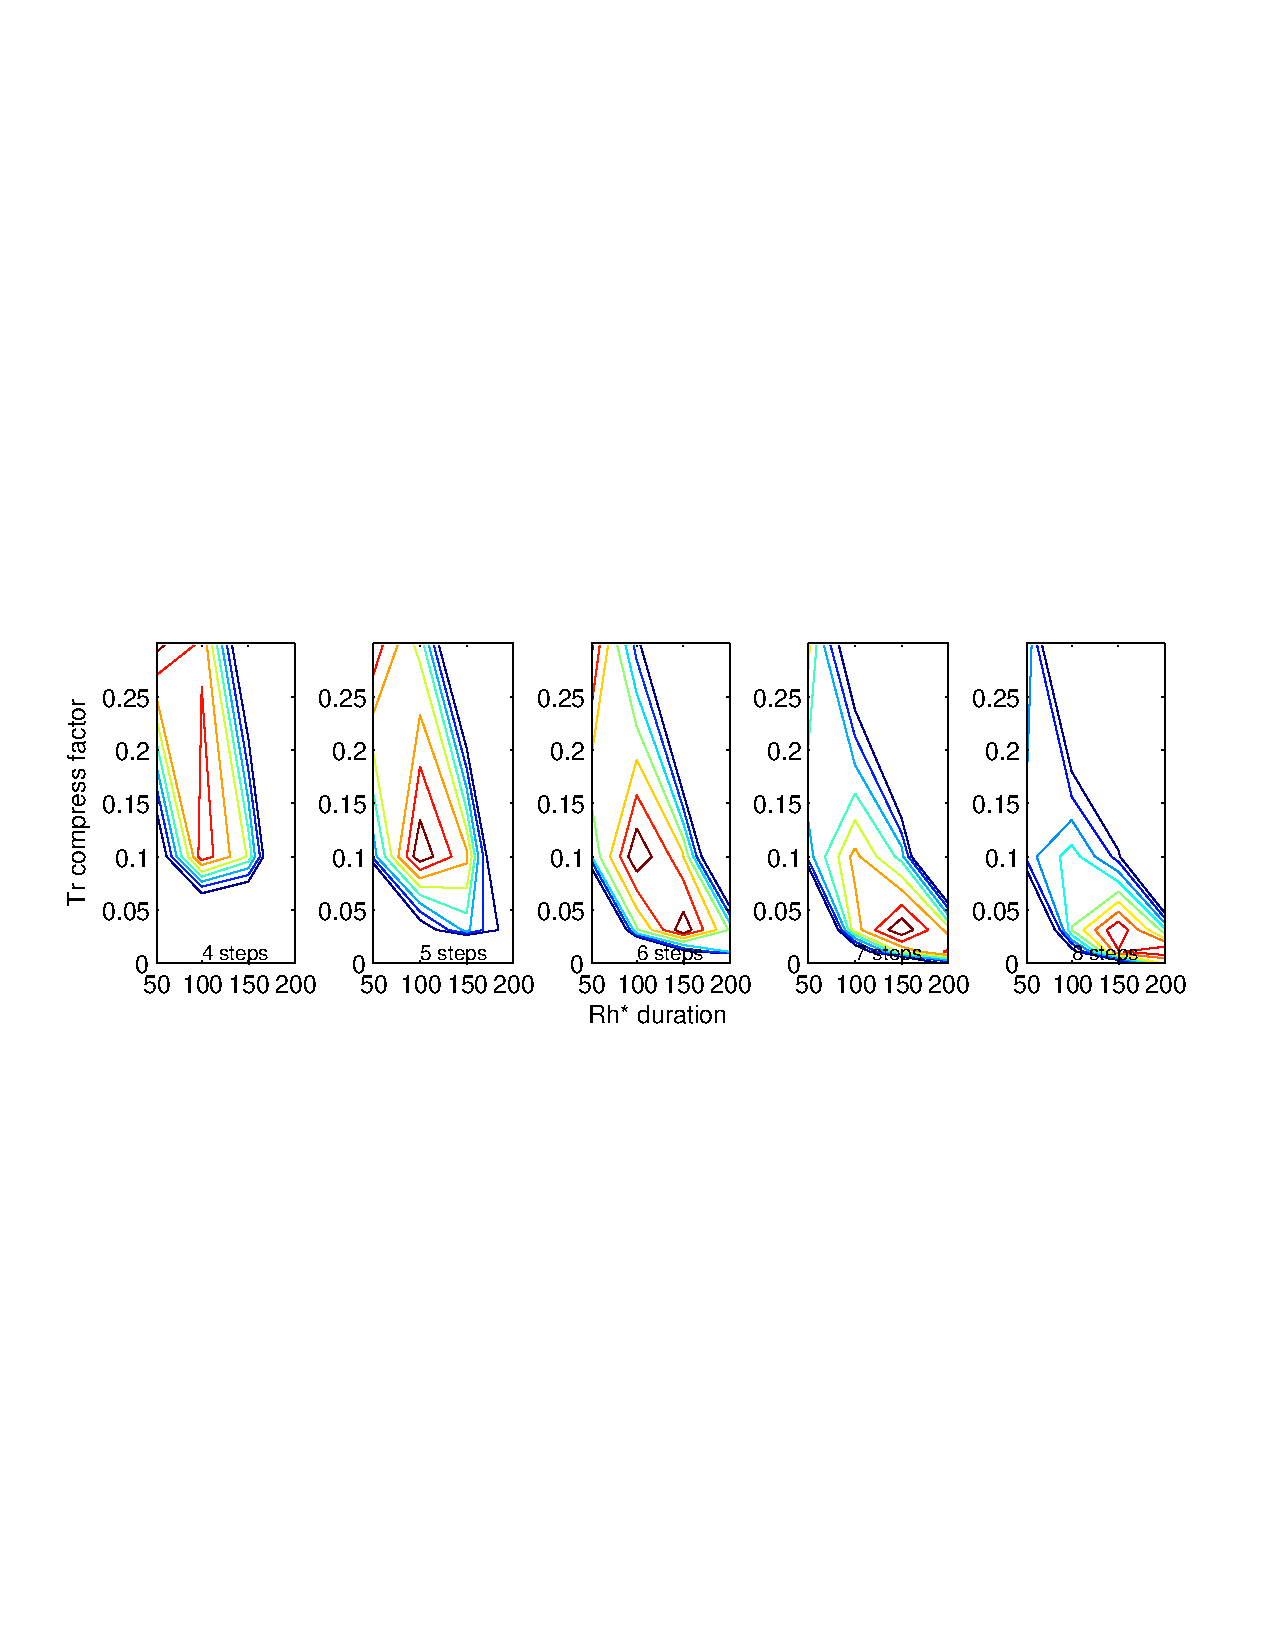
\includegraphics[width=6in]{TrCompression.pdf}
\caption{Likelihood analysis of models with transducin compression.}
\label{fig:TrCompression}
\end{center}
\end{figure}

Compression of transducin activity could also trade with the number and duration of shutoff steps for \GCAPKO responses.  With a substantial reduction in the number of inactivation steps, somewhat different combinations of parameters were required to maximize likelihood for \GCAPKO and wild-type responses.  For example, for 4 inactivation steps and some transducin compression, likelihood for \GCAPKO responses was maximized for a rhodopsin duration of 310 ms.  Forcing the rhodopsin duration to match that of wild-type responses decreased likelihood 3-5-fold.  

Models in which transducin activity was subject to substantial compression poorly captured the amplitude of single photon responses generated by rhodopsin lacking phosphorylation sites.   We repeated the analysis of Figure~\ref{fig:linear-predict} for models with different degrees of transducin compression.  Figure~\ref{fig:TCompressCSM} plots likelihood obtained by comparing model predictions with the mean and SEM of the no-phosphorylation site responses.  Values of transducin compression that permitted a substantial reduction in the number of shutoff steps (e.g. Figure~\ref{fig:TrCompression}) poorly (likelihood $<$ 0.01) captured the CSM responses.  

\begin{figure}[h]
\begin{center}
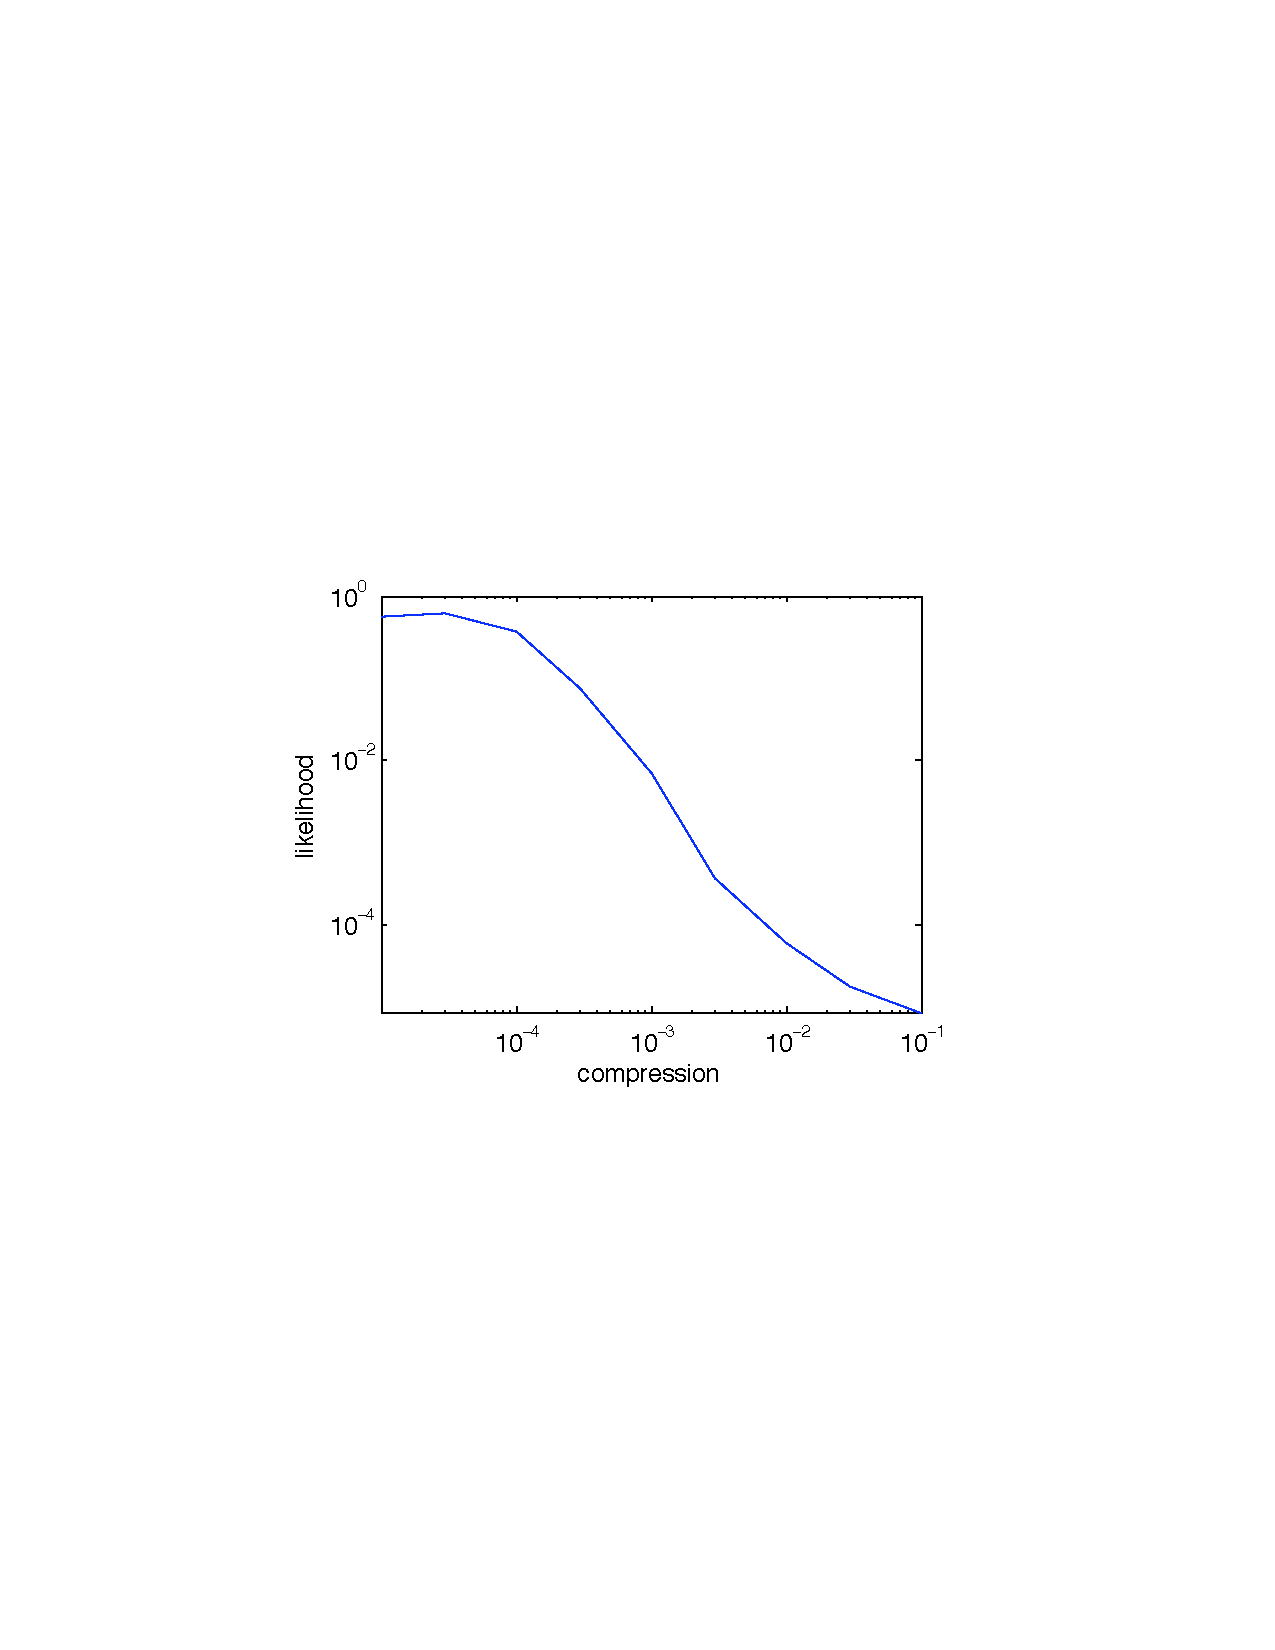
\includegraphics[width=2.5in]{TCompressCSM.pdf}
\caption{Likelihood analysis of CSM response amplitude for different degrees of transducin compression.}
\label{fig:TCompressCSM}
\end{center}
\end{figure}


%%%%%%%%%%%%%%%%%%%%%%%%%%%%%%%%%%%%%%%%%
%%%%%%%%%%%%%%%%%%%%%%%%%%%%%%%%%%%%%%%%%
%%%%%%%%%%%%%%%%%%%%%%%%%%%%%%%%%%%%%%%%%

\vfill\eject

\section{Notes and Results}

\subsection{Collected experimental measures of response variability}

\begin{figure}[h]
\begin{center}
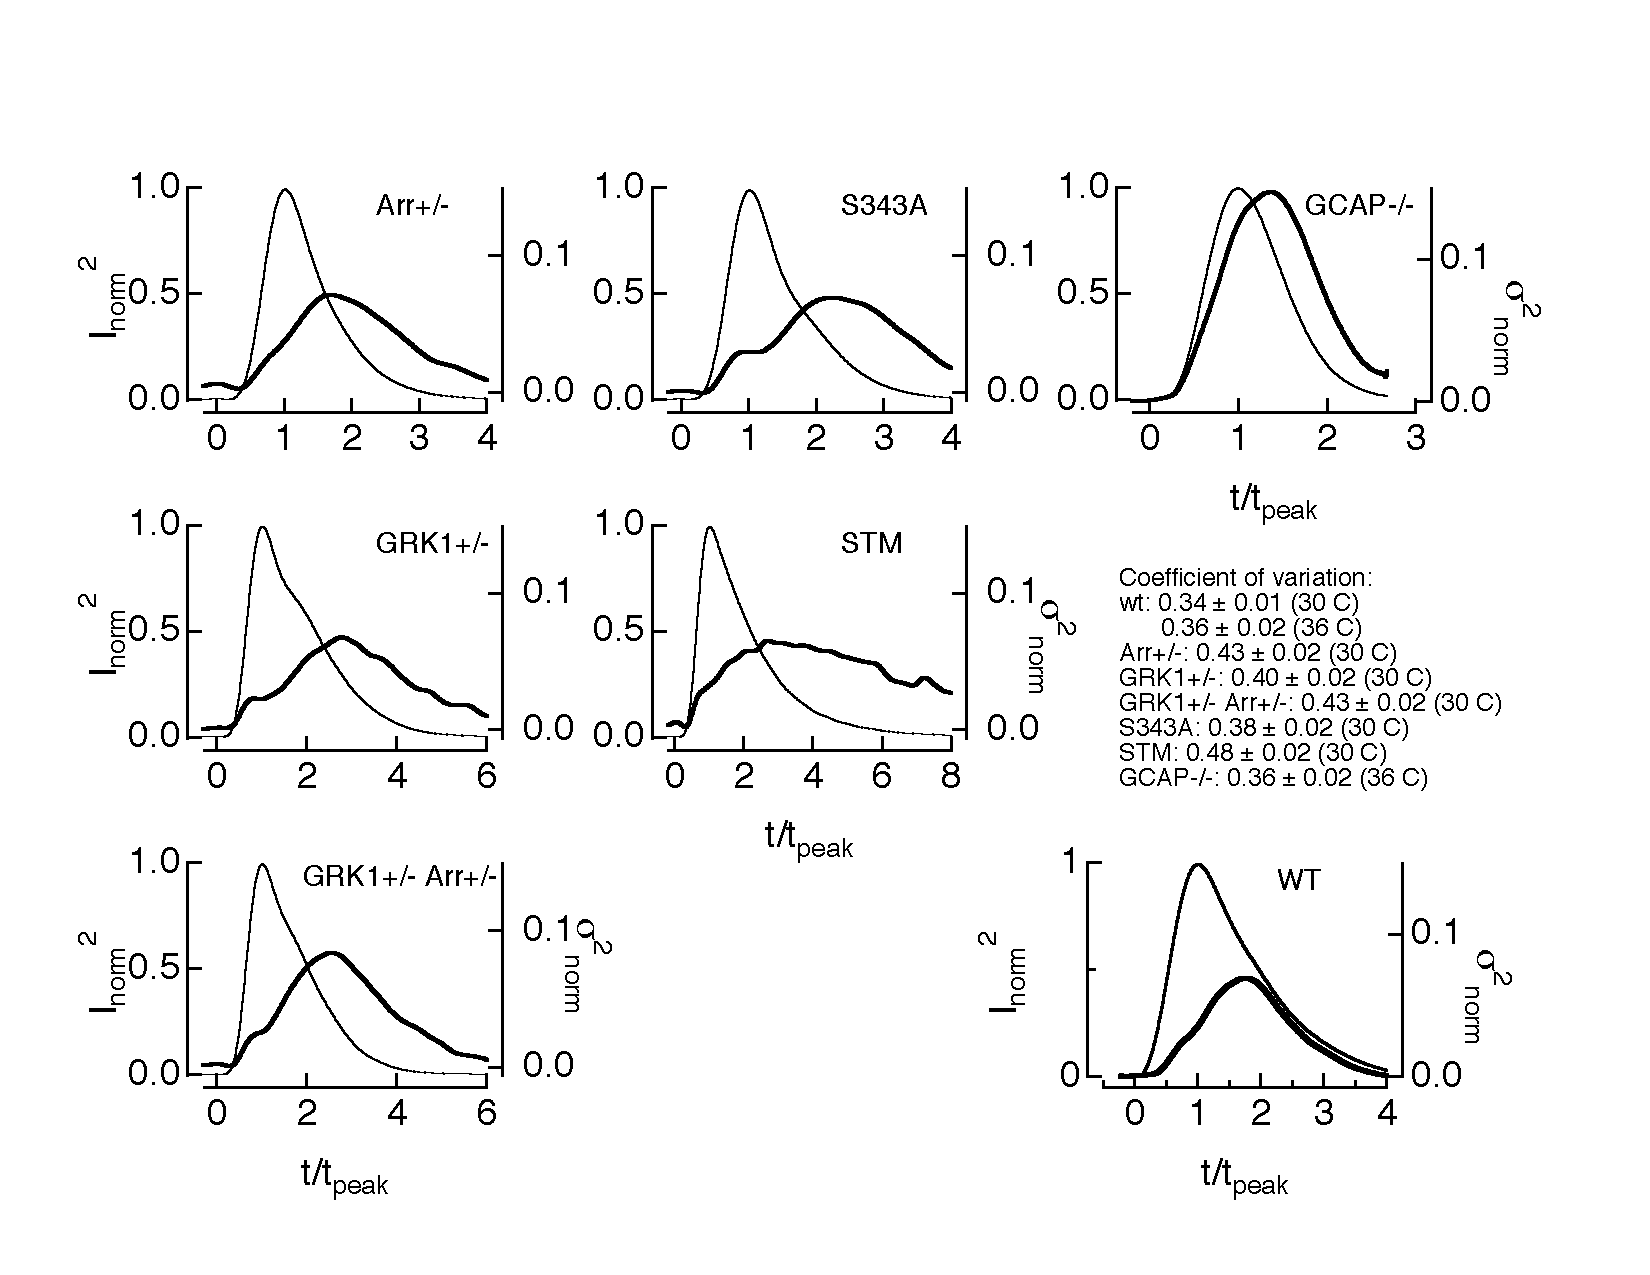
\includegraphics[width=6in]{repro_zoo.pdf}
\caption{Square of mean response and time-dependent variance for various genetic manipulations.}
\label{fig:repro_zoo}
\end{center}
\end{figure}

We have measured variability of single photon responses from a number of transgenic mice (Figure \ref{fig:repro_zoo}).  These are summarized here, with some caveats about the transgenic approach.

\bi

\i{{\bf Phosphorylation site mutants.}  Response variability changes systematically with reduction in the number of phosphorylation sites.  It is difficult to compare the response kinetics with wt because of differences in pigment expression level, which effect response kinetics (e.g. Calvert Rh$^{+/-}$ paper).  Most of this is published in Doan et al (2006).}

\i{{\bf GCAP$^{-/-}$.}  Responses are large and could be compressed --- thus low variability could be increase due to lack of calcium feedback and decrease due to compression.  No evidence for this though as filter that explains change in noise explains change in response (Burns 2002) --- we need to check this ourselves and for our recording conditions.  These results are not published.}  

\i{{\bf Arr$^{+/-}$ and GRK1$^{+/-}$.}  Unclear how reduction in both arrestin and kinase results in responses with very similar kinetics to wt, but increased variability.  Suggests disruption of timing across shutoff steps.}

\ei

What do we want to model here?  Some thoughts:

\bi

\i{Comparison of GCAP$^{-/-}$ and wt is interesting re role of calcium feedback to cyclase in suppressing variability.  This seems a straightforward model --- can a single model for rhodopsin inactivation, coupled to different deterministic models for the transduction cascade, account for change in single photon response and in time-dependent variance?  Could throw in GCAP$^{+/-}$ results (would need to collect them).  Take approach similar to that below --- assume rhodopsin and PDE have same properties, derive filters, predict mean and time-dependent variance for both wt and GCAP knockouts, identify parameters most consistent with data.}

\i{What do we get from comparison of responses in different recording conditions?  Can we use those measurements to (a) constrain transduction cascade?  (b) Constrain models for reproducibility?  In particular, are there conditions in which single photon responses vary only in amplitude (L15/Locke's - GCAP$^{-/-}$)?}  

\i{Can we model interactions of arrestin, kinase and transducin?}

\ei

\subsection{Predicting response amplitude and kinetics assuming linear transduction process}



\begin{figure}[h!]
\begin{center}
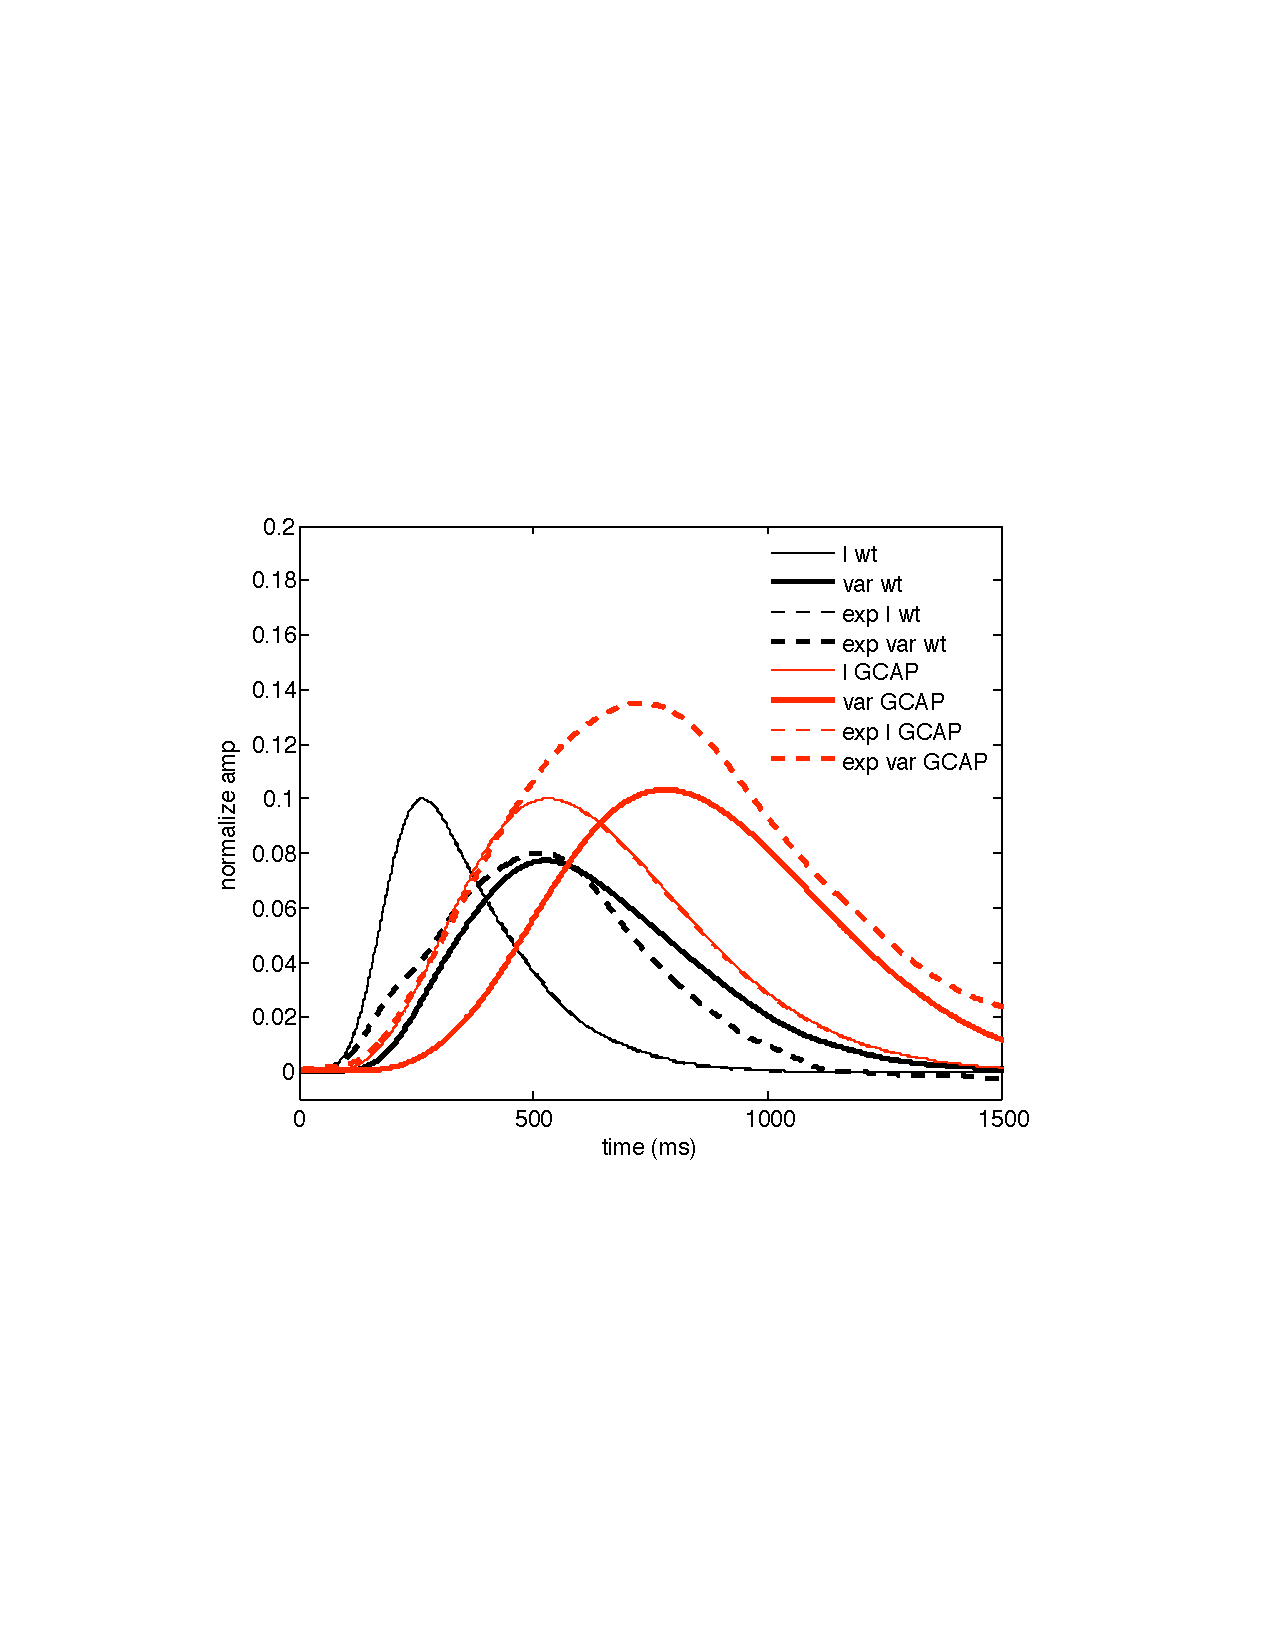
\includegraphics[width=3in]{GCAPKOFullKinetics.pdf}
\caption{Predicted time-dependent variance for wt and \GCAPKO rods assuming rhodopsin inactivation time constant of 300 ms, multistep shutoff with equal decay in activity for each step.}
\label{fig:GCAPFull}
\end{center}
\end{figure}

\begin{figure}[h!]
\begin{center}
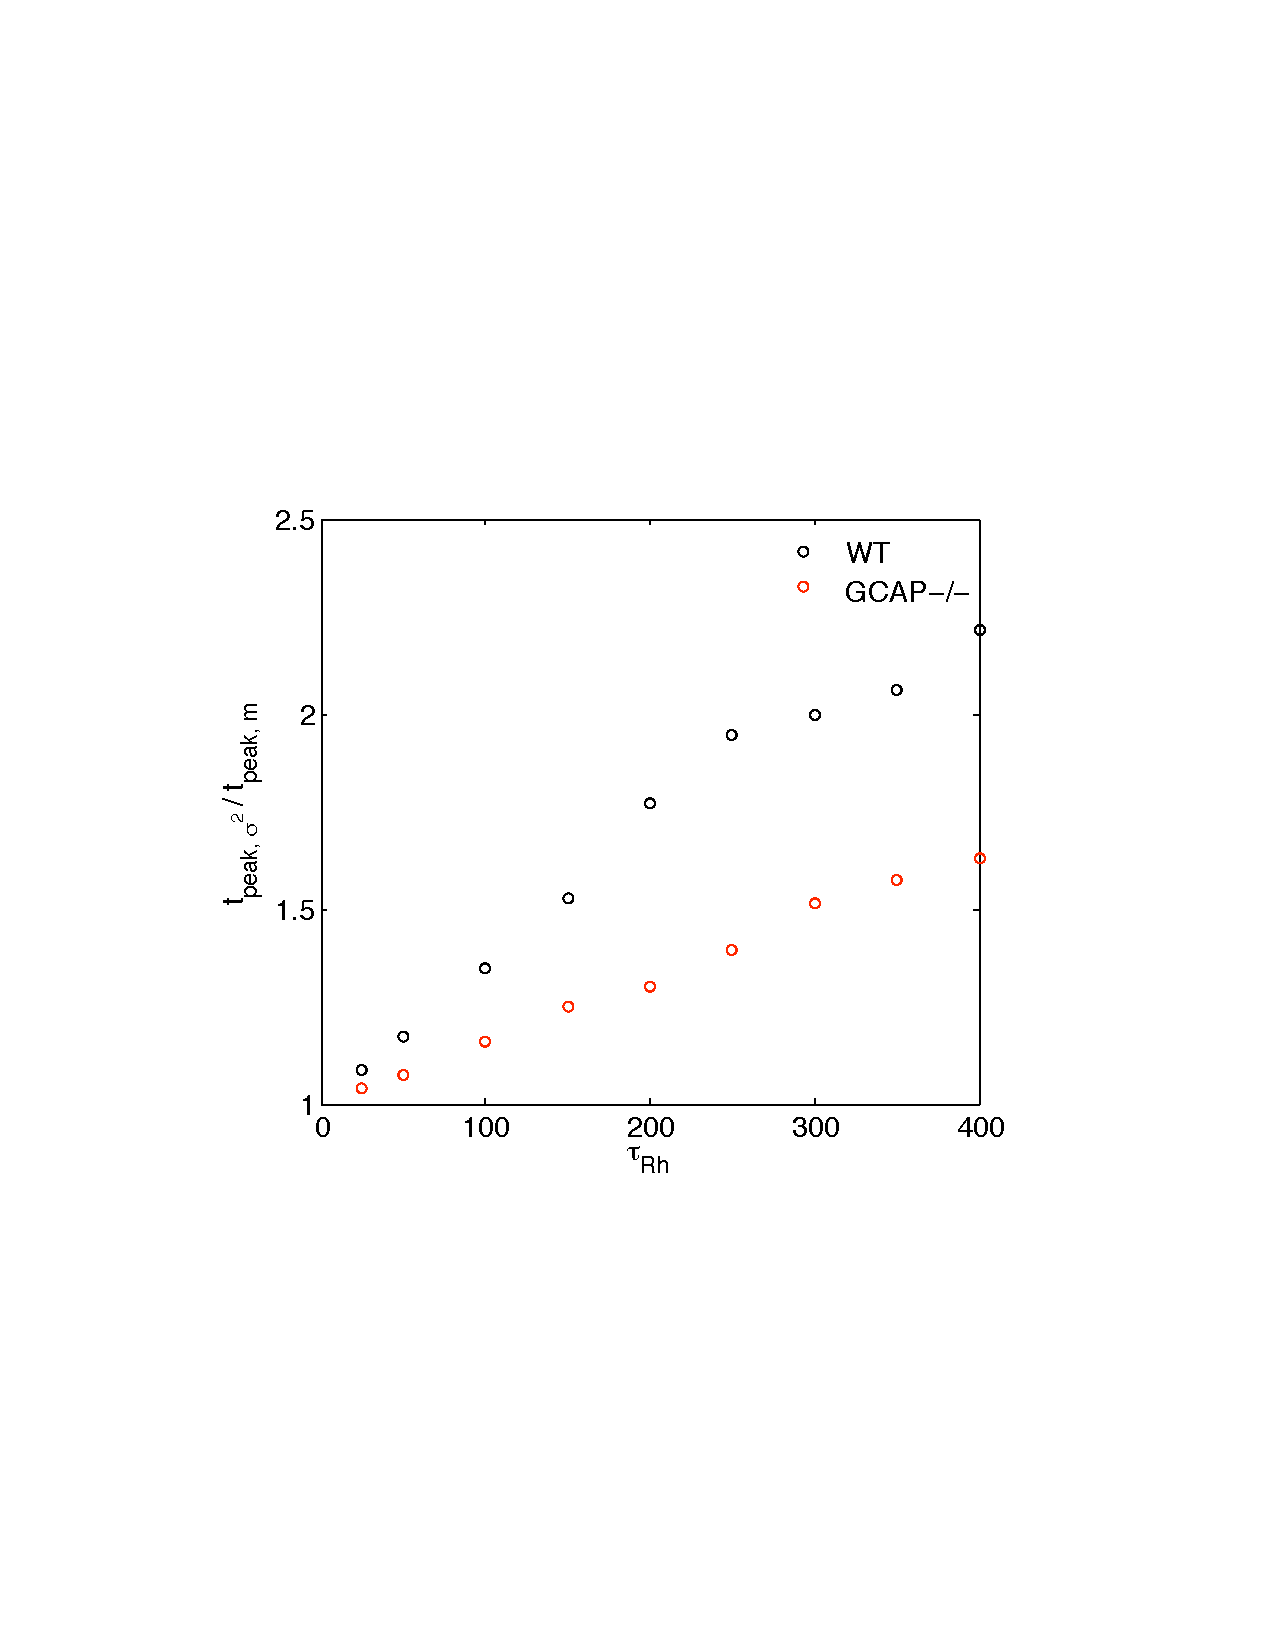
\includegraphics[width=3in]{GCAPKOKinetics.pdf}
\caption{Predicted \tpeakratio for wt and \GCAPKO rods for multiple Rh* inactivation time constants.}
\label{fig:GCAP}
\end{center}
\end{figure}

\begin{figure}[h]
\begin{center}
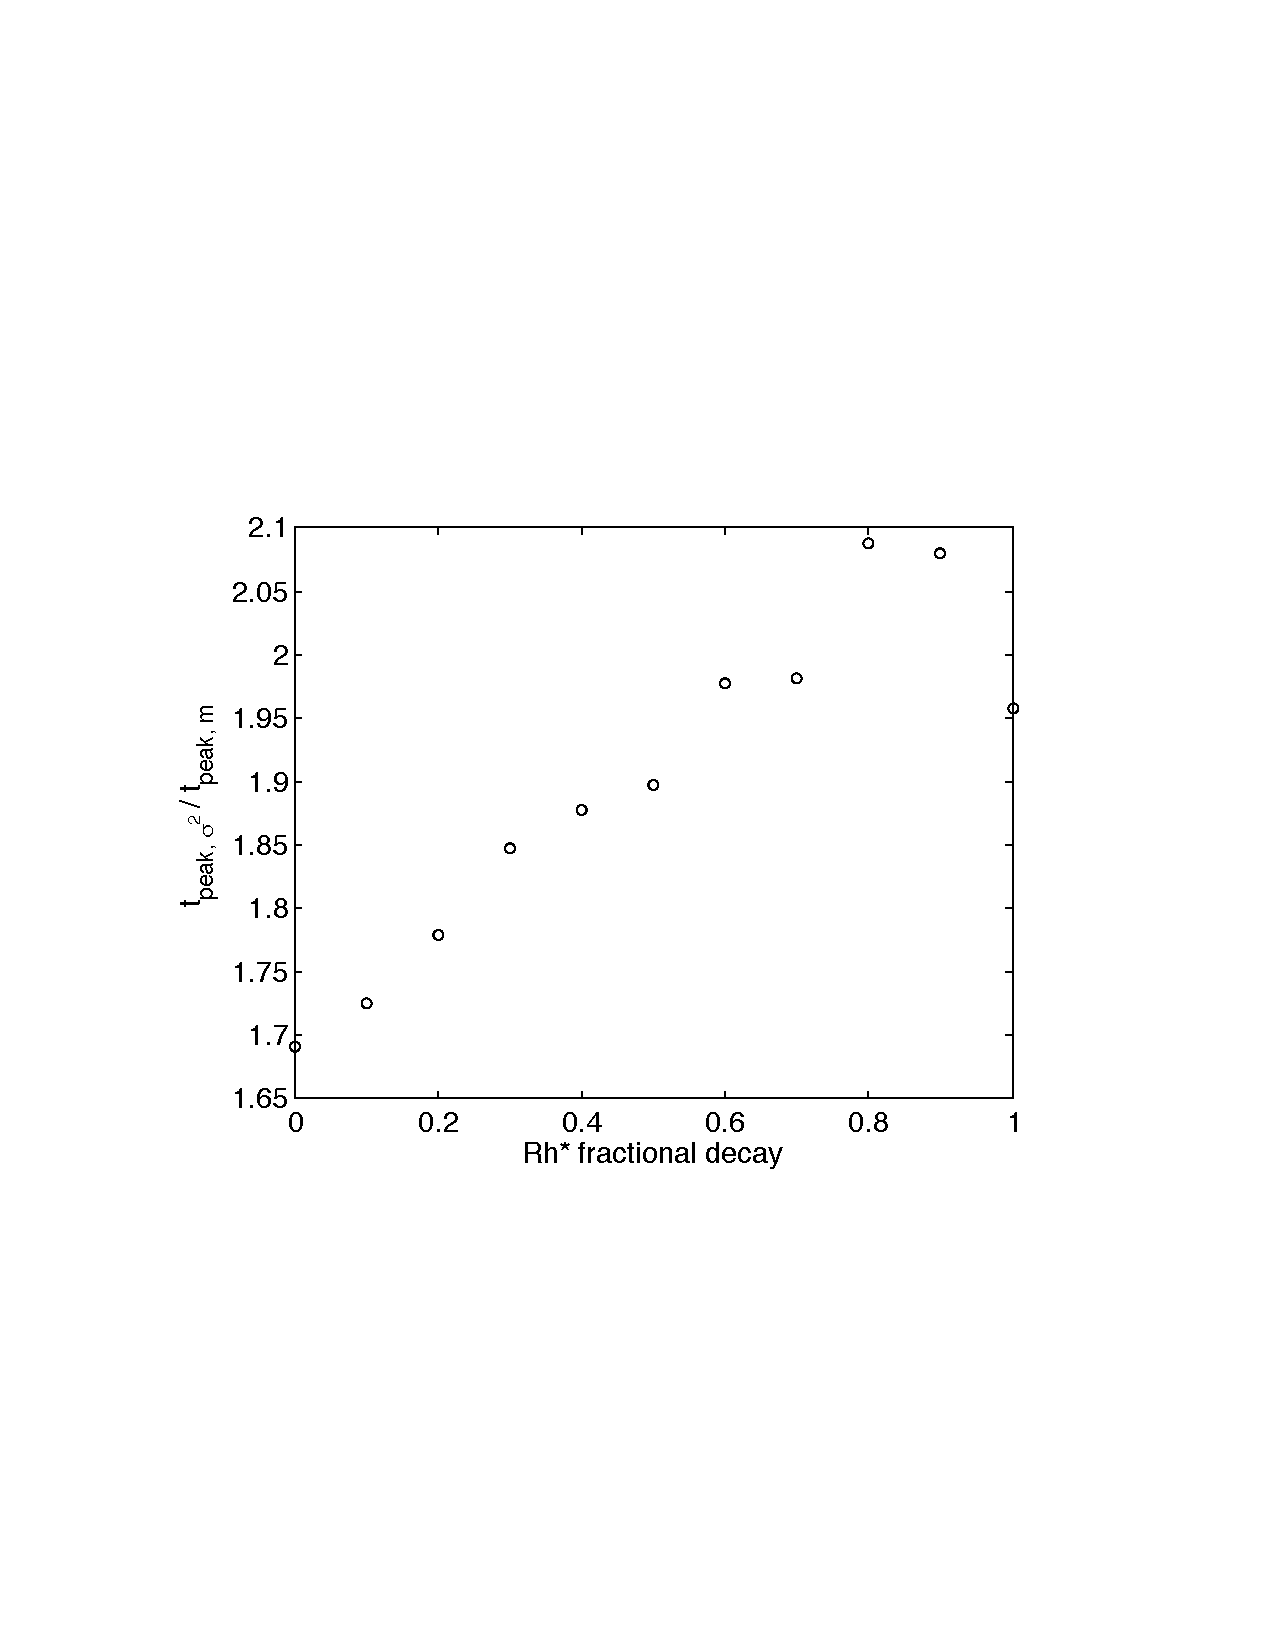
\includegraphics[width=3in]{decay-shape.pdf}
\caption{Predicted \tpeakratio for wt rods as a function of $\Delta$, which controls the degree to which Rh* inactivation is gradual or abrupt.}
\label{fig:decay-shape}
\end{center}
\end{figure}

\begin{figure}[h]
\begin{center}
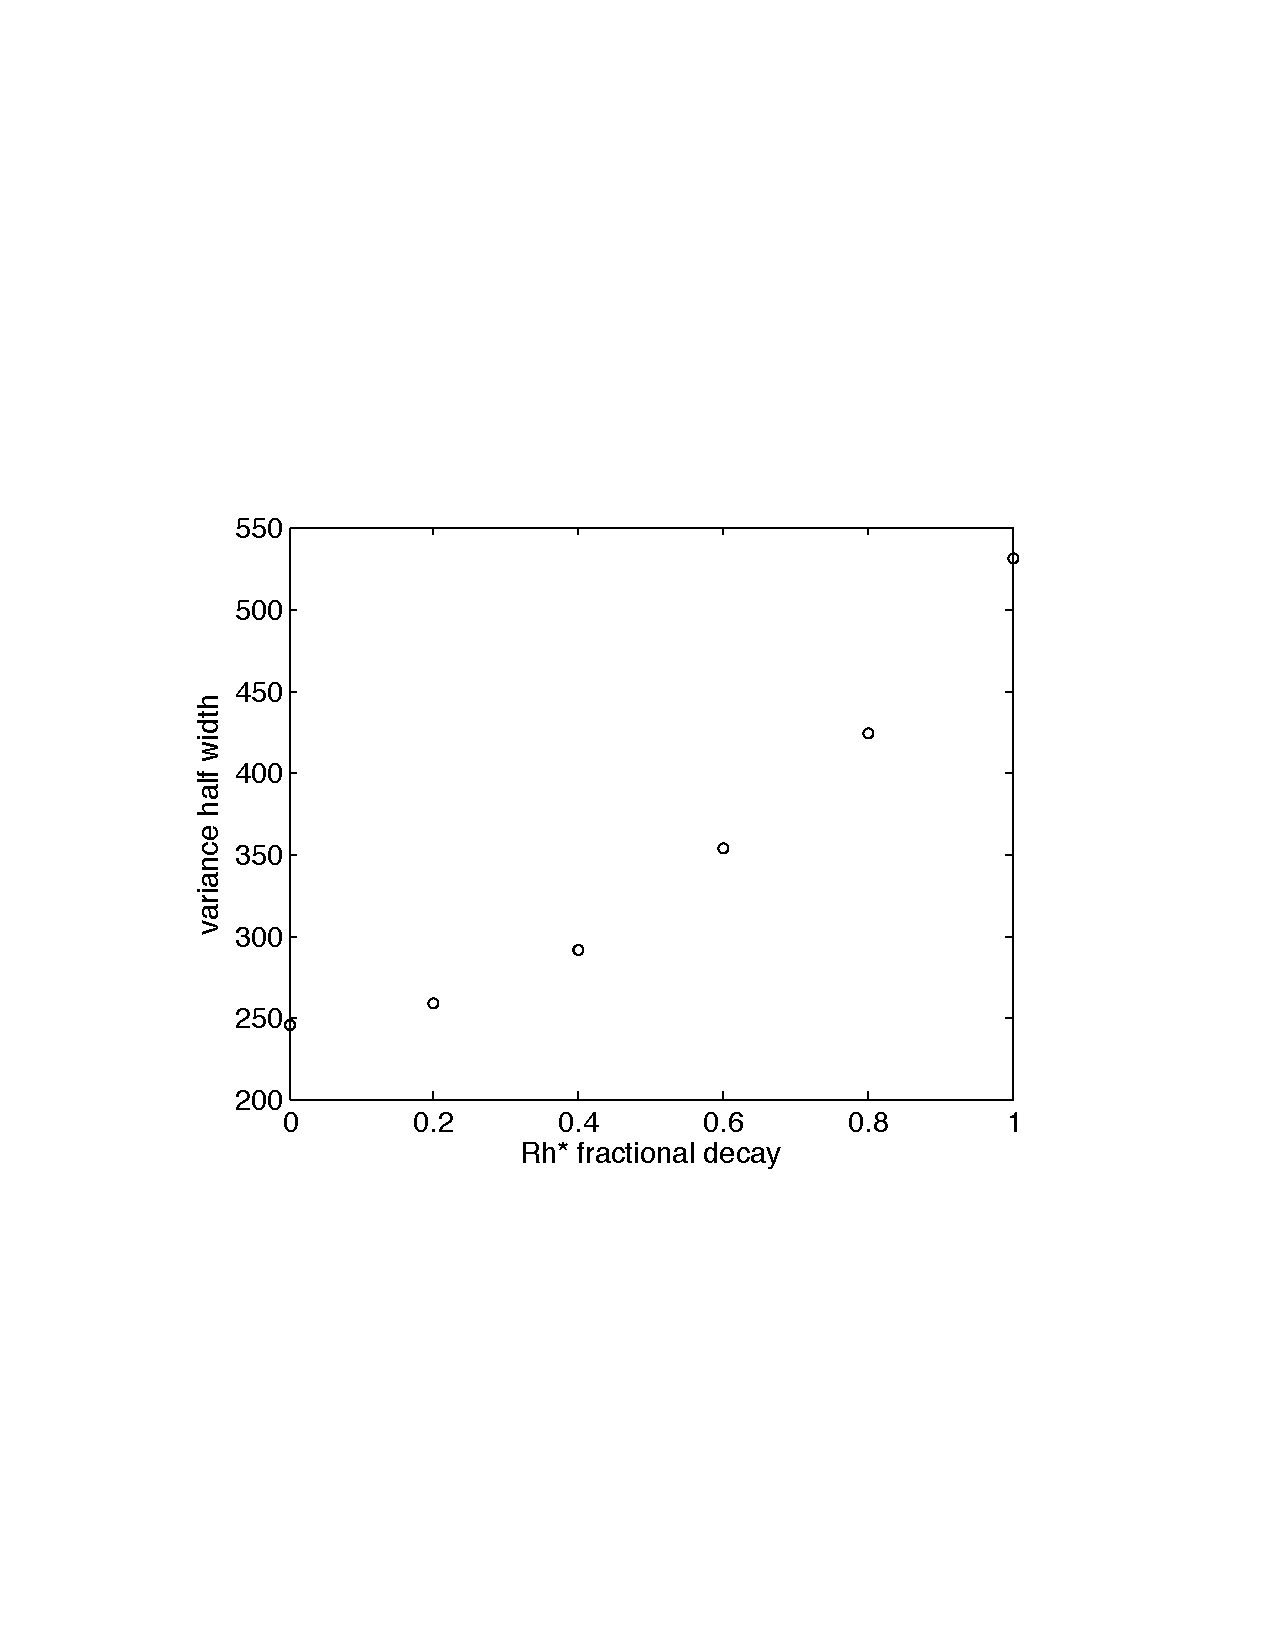
\includegraphics[width=3in]{decay-var-width.pdf}
\caption{Predicted variance with (full width at half max) for wt rods as a function of $\Delta$, which controls the degree to which Rh* inactivation is gradual or abrupt.}
\label{fig:decay-shape}
\end{center}
\end{figure}

\begin{figure}[h]
\begin{center}
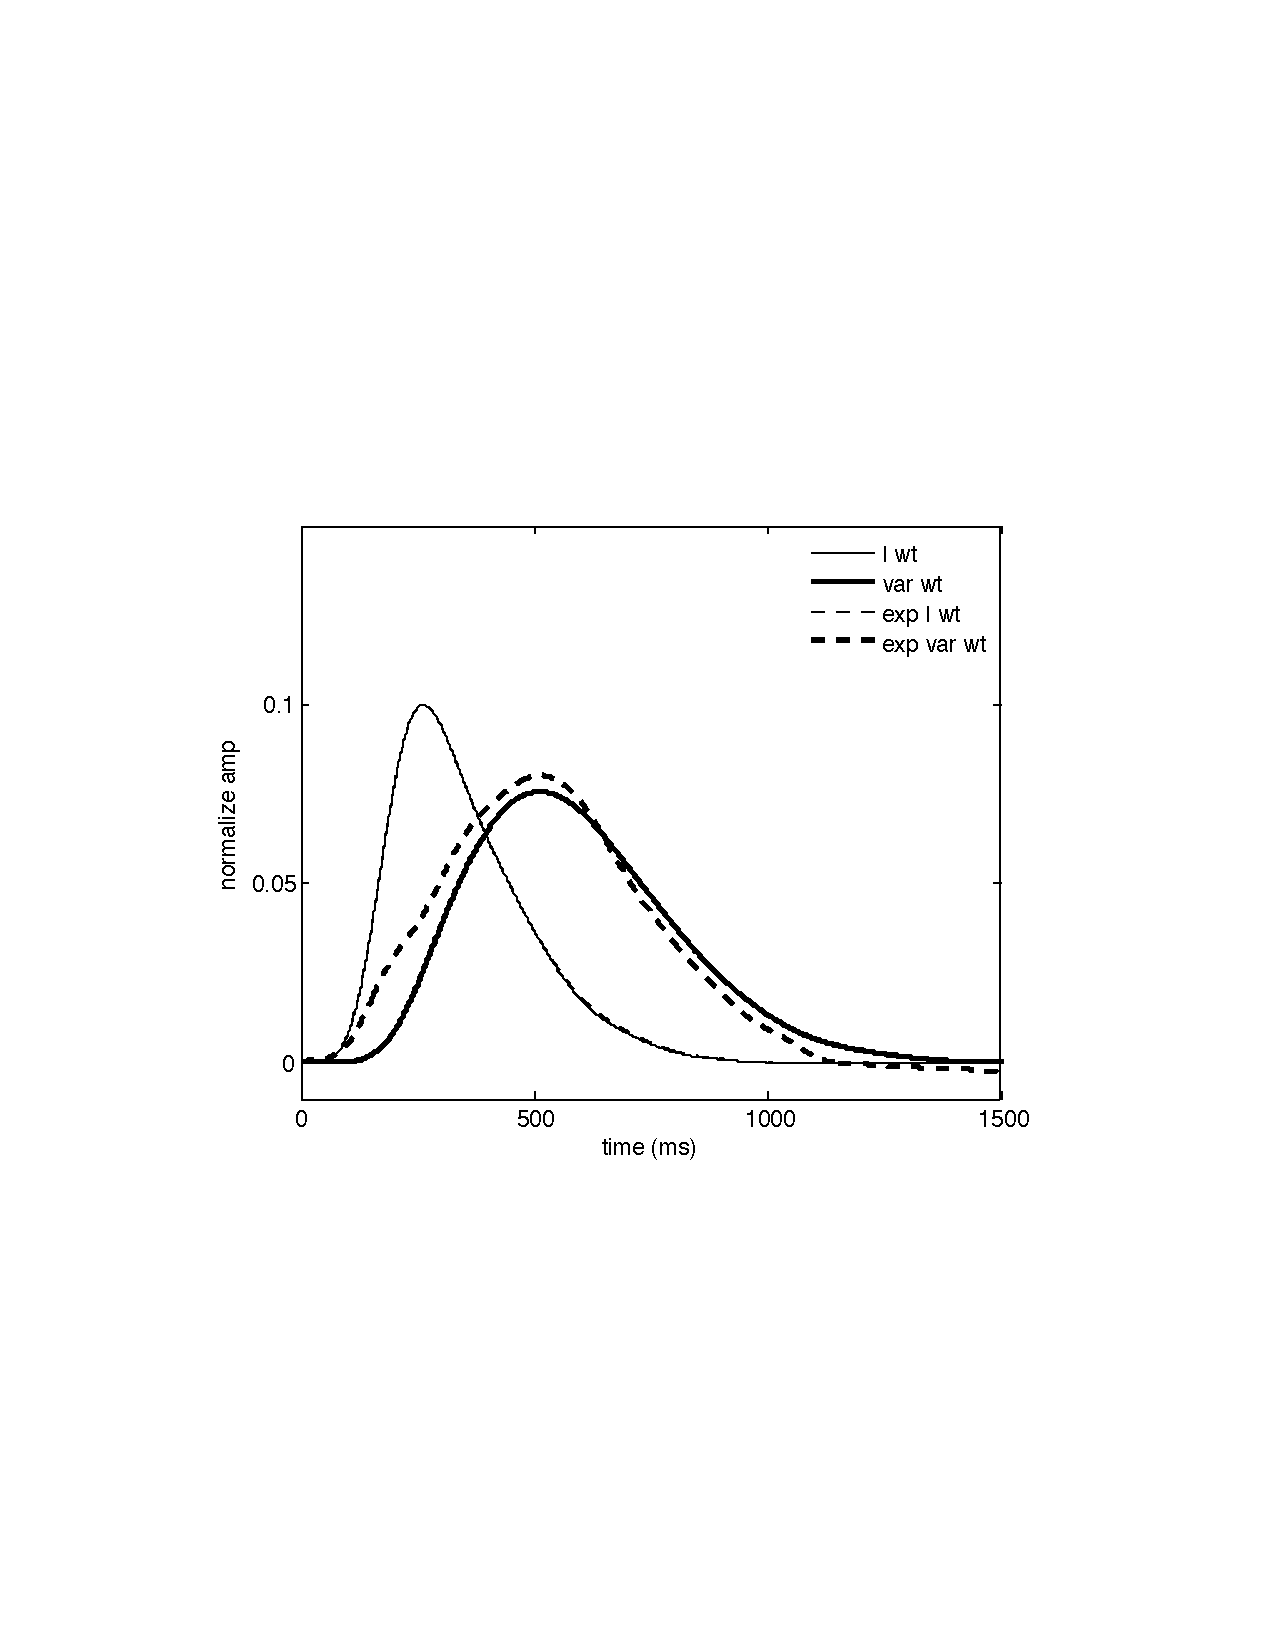
\includegraphics[width=3in]{wt-delta1.pdf}
\caption{Predicted time dependent variance for $\Delta = 1$.}
\label{fig:delta1}
\end{center}
\end{figure}

\begin{figure}[h]
\begin{center}
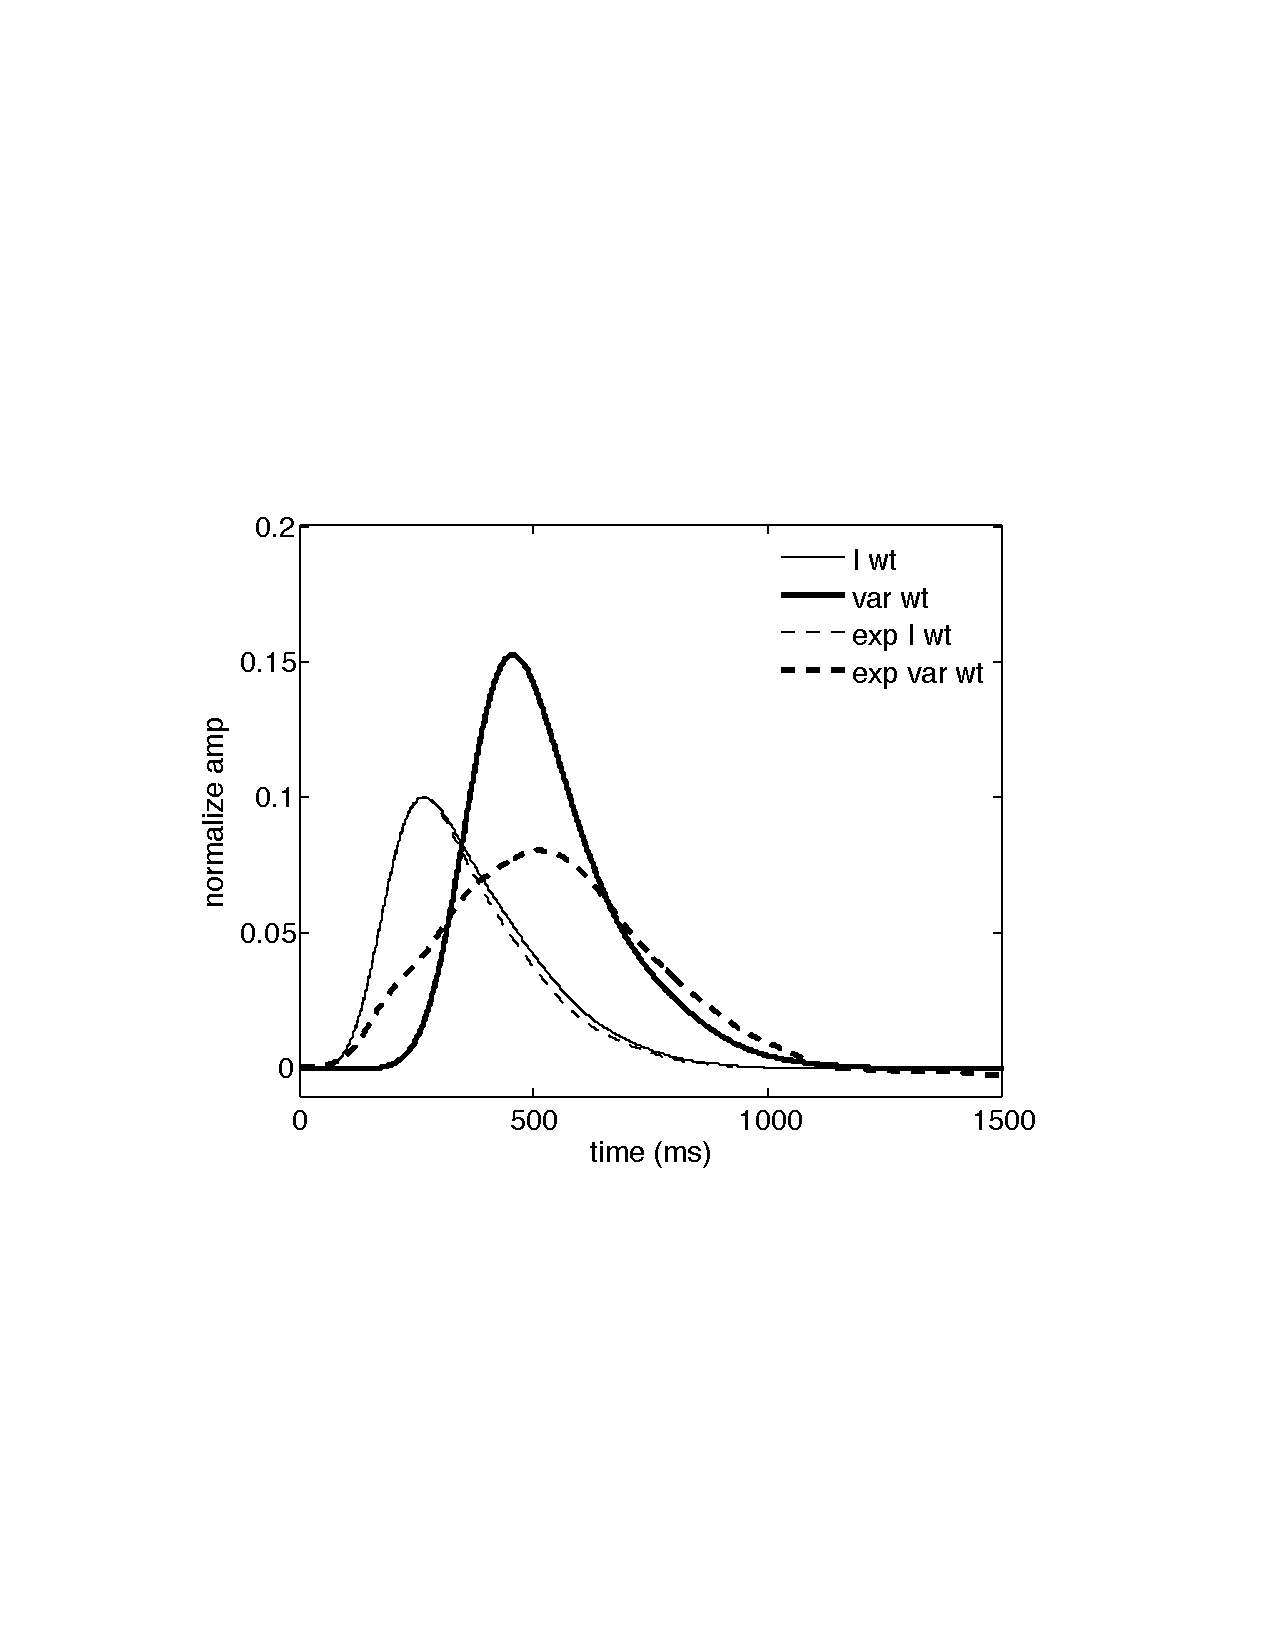
\includegraphics[width=3in]{wt-delta0.pdf}
\caption{Predicted time dependent variance for $\Delta = 0$.}
\label{fig:delta0}
\end{center}
\end{figure}



NOTE: need to fix time-dependent variance in Fig.~\ref{fig:GCAPFull} and below to use normalized time.  See Fig.~\ref{fig:repro_zoo}.

\subsection{Fitting time-dependent variance of \GCAPKO~and wt responses}

If the transduction process is linear and \Ca feedback does not suppress variability, then variability in the responses of \GCAPKO rods should be predictable from that of wild-type rods.  This could fail because of: (1) saturation at or downstream of the PDE (i.e. saturation created by larger change in cGMP concentration in \GCAPKO~vs wt rods); or (2) because \Ca feedback regulates response variability.  

Assume as above that the transduction process is linear.  Use the average single photon responses for both \GCAPKO~and wt rods to derive linear filters approximating the transduction cascade for a given decay-model for Rh* inactivation.  Now use multistep model and these linear transduction filters to estimate how time-to-peak of variance relative to mean depends on $\tau_{Rh}$.  

Experiment:  wt \tpeakratio = 1.96 and \GCAPKO~\tpeakratio = 1.38.  \CVArea is quite similar for both.

With $N = 8$ and $\Delta = 1$ (see next section), models with $\tau_{Rh} \approx 300-350 ms$ capture both of these pretty well (see Figs.~\ref{fig:GCAPFull} and \ref{fig:GCAP}). The exact value of $\tau_{Rh}$ that provides best match depends on the number of steps.  Some dependence on $\Delta$ but not that strong (see below for more detailed analysis of $\Delta$).

\subsection{Rh* inactivation: Flat vs gradual decline}

Generate set of models as above where Rh* activity following each step is
\begin{equation}
Rh^*_n = Rh^*_0  (1 - n\Delta/N)
\end{equation}
and rate constant for step is
\begin{equation}
\alpha_n = \alpha_0  (1 - n\Delta/N).
\end{equation}
$\Delta$ sets rate of decline in activity ($\Delta = 0$ means activity flat until final step, $\Delta = 1$ means staircase with equal steps).  

Capture time-dependent variance pretty well as long as $\Delta > 0.6$ (see Figure \ref{fig:decay-shape}).  In general time to peak of variance not that sensitive to $\Delta$, but shape of predicted variance is quite sensitive (i.e. when $\Delta$ is small, width of variance small --- see Figs.~\ref{fig:delta1} and \ref{fig:delta0}).  Experimental width is $\sim$ 500 ms.

\subsection{Model with stochastic transducin activation}

What constraints does variability of single photon response place on transducin activation?  To explore this issue, consider models with stochastic transducin activation.  As first step, measure \CVArea for model with 8 step Rh* inactivation (theoretical \CVArea = 0.35) as a function of transducin activation rate.  Fig.~\ref{fig:transducin} shows result.  Assuming linearity of transduction process, explaining experimental \CVArea requires 50-100 transducins to be activated by single Rh*.  Need $\sim$ 20 transducins if Rh* inactivation is deterministic.

Stochastic transducin activation also does not appear to capture the late time to peak of the time-dependent variance.  The variability introduced has a shape very similar to the mean response itself, so a model with a brief Rh time course and long transducin time course has a time-dependent variance with a shape very similar to the mean squared response itself.

\begin{figure}[h]
\begin{center}
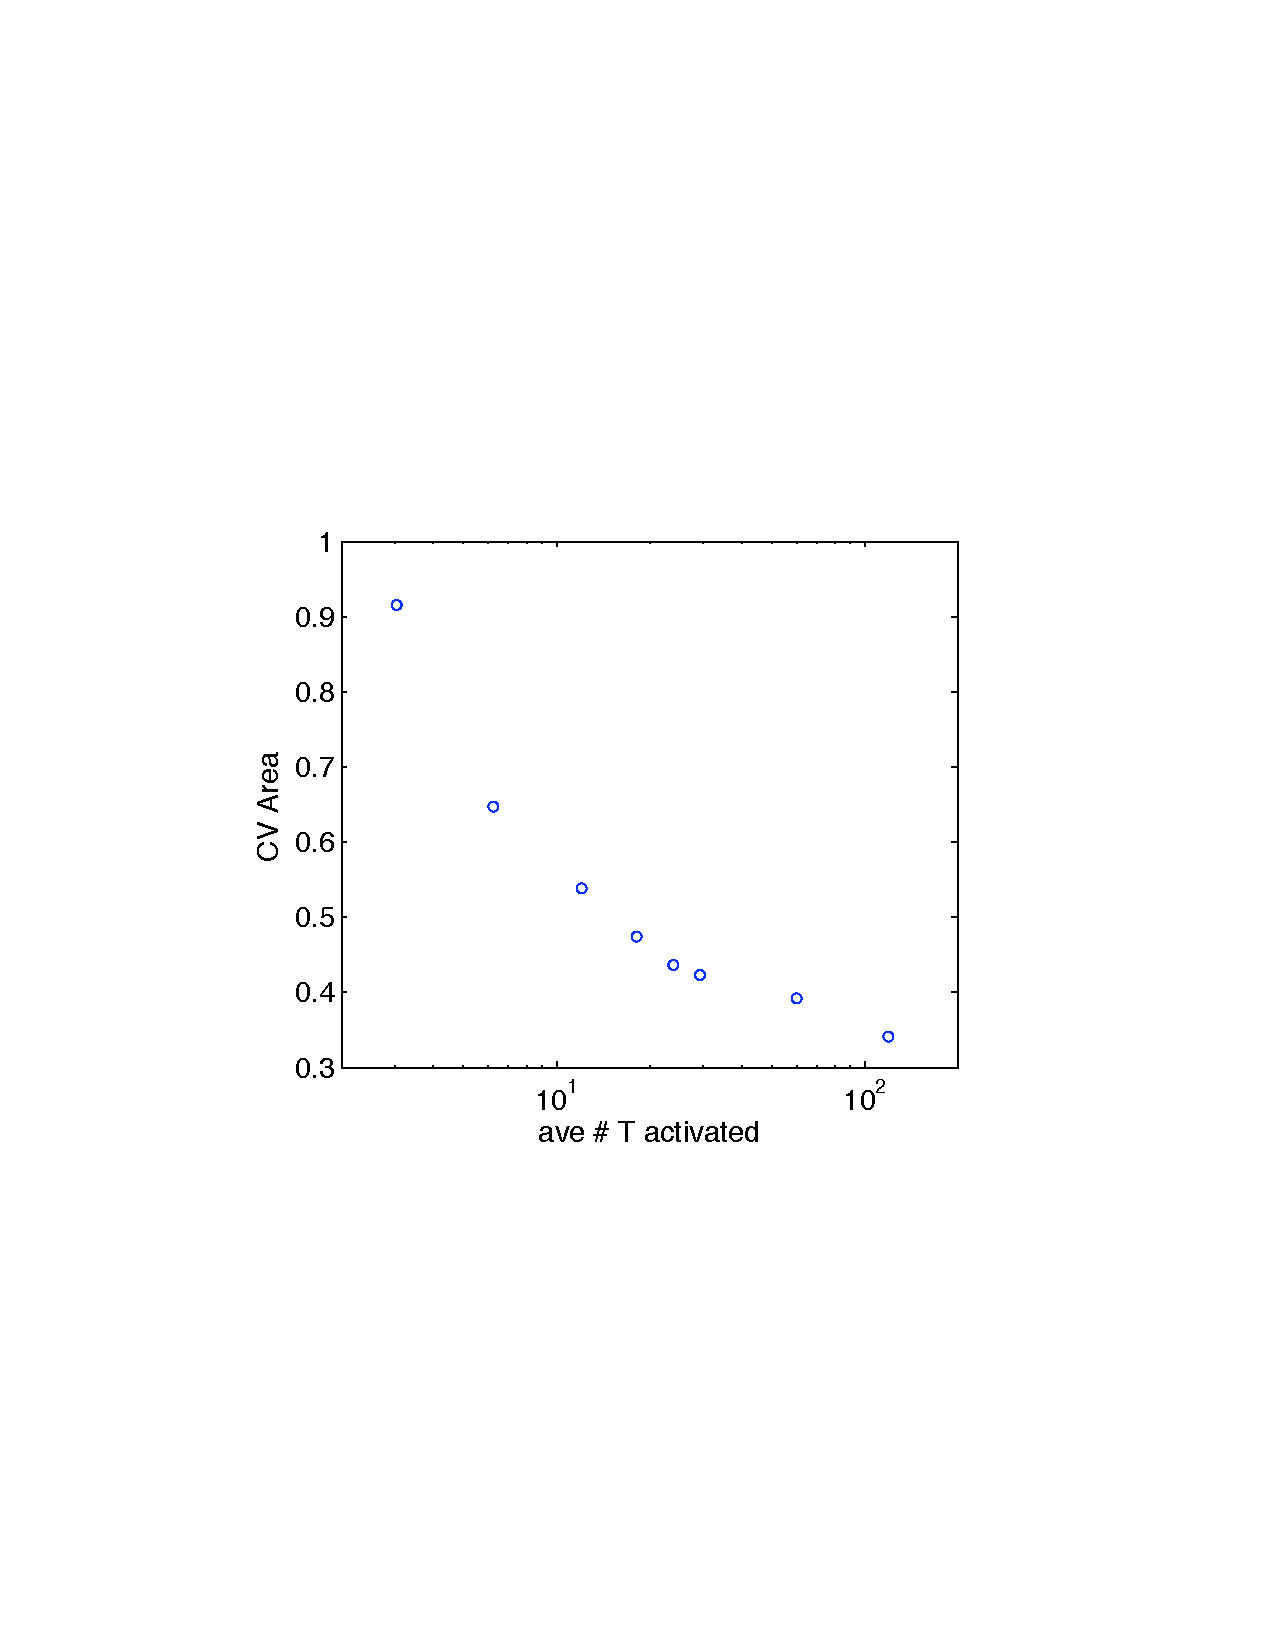
\includegraphics[width=3in]{transducin.pdf}
\caption{\CVArea for models with stochastic transducin activation.  Rh model was 8 step shutoff with $\Delta = 1$.}
\label{fig:transducin}
\end{center}
\end{figure}

\subsection{Nonlinear transduction process}

%%%%%%%%%%%%%%%%%%%%%%%%%%%%%%%%%%%%%%%%%

\vfill\eject

\section{Some (older) random notes}

\subsection{Properties in need of explanation}

\bi

\i{CV$_{area} \approx $ 0.35}

\i{late time-to-peak of time-dependent variance}

\i{sensitivity of CV$_{area}$ to manipulations targeting rhodopsin inactivation - deletion of phosphorylation sites, alteration in kinase and/or arrestin concentrations.}

\i{insensitivity of CV$_{area}$ to manipulations targeting late steps in transduction --- e.g. loading cells with BAPTA, deletion of GCAP, ...}

\i{lack of interaction of single photon responses delivered in local ($\sim 1 \mu$m) region of outer segment (Field and Rieke)}

\i{Rieke and Baylor gain experiments - reducing gain by manipulating GTP/GDP ratio did not alter kinetics of response.  Can we repeat this in mouse?  Caveat of truncated cells.}

\ei

\subsection{Models to consider}

\bi

\i{very simple model with no kinetics about importance of statistics of transducin activation and noise produced by transducin --- all re CV$_{area}$.}

\i{linear cascade model with multi-step rhodopsin inactivation}

\i{cascade model with nonlinearity in disc-associated reactions, multi-step rhodopsin inactivation (see Detwiler and Shraiman).}

\i{cascade model with nonlinearity in reactions coupling disc to surface membrane, multi-step rhodopsin inactivation (similar to Bisegna).}

\ei

Questions:

\bi

\i{How mechanistically detailed should we make model --- e.g. include specific inactivation events, or leave them as ``steps'' without specification of origin?  Similarly nonlinearities --- can we make genetic disc-associated and diffusive nonlinearities without getting into which components involved?}

\i{What is spatial profile of reduction in cGMP produced during single photon response?  Nonlinearities in transduction process produced by depletion of cGMP in vicinity of activated PDE could reduce variability.  Does cGMP synthesized by GC ``invade'' intradiscal space; if so would expect that nonlinearity due to cGMP depletion would be exacerbated in GCAP knockouts or rods loaded with BAPTA.}


\ei

\subsection{Relevant experimental results}

\bi

\i{Evidence for linearity of transduction process

\bi

\i{GCAP$^{-/-}$ responses in Burns 2002.  Linear filter that explains difference in light response of wt and GCAP$^{-/-}$ rods can also account for difference in continuous noise.  This speaks specifically to linearity of calcium feedback to cyclase.  }

\i{Responses to two nearby photons add linearly (Field 2002).  Flashes delivered through slit $\sim$1-2 $\mu$m in width summed linearly up to 5-6 Rh*.  This region contains 50-100 discs, so test is for nonlinearities in coupling of disc activity to channels.  This could include nonlinearities in effective PDE activity if change in cGMP produced at one disc extends to nearby discs.  }

\i{Success of linear models in capturing response (acknowledge uniqueness has not been dealt with).}

\ei

}

\i{Importance of feedback

\bi

\i{Rieke and Baylor gain experiments - reducing gain by manipulating GTP/GDP ratio did not alter kinetics of response.}

\i{\Ca feedback.  Burns and Baylor loaded GCAP$^{-/-}$ rods with BAPTA and saw little or no change in response.   \Ca feedback other than that mediated by GCAP should be altered by BAPTA.}

\i{more \Ca feedback.  In Field and Rieke (2002) we loaded cells with BAPTA and found little change in response variability.}

\ei

}

\ei


\subsection{New experimental tests}

\bi

\i{variability in responses of GCAP$^{-/-}$ rods.  Caveat is that these responses are large - could they be saturated?  Test: cross GCAP$^{-/-}$ rods into Arr$^{+/-}$ or GRK1$^{+/-}$ background and see if additional variability intact --- i.e. should see similar increase in variability seen starting from wt if responses are not saturated.}

\i{linearity.  Repeat Burns et al. (2002) test for: (1) linearity of calcium feedback by comparing continuous noise and single photon responses in wt and GCAP knockout mice; (2) lack of other significant calcium feedback pathways by loading GCAP knockout rods with BAPTA and testing for effect on single photon response kinetics and variability.}

\i{rgs9 overexpressing rods?  If we can measure responses these would provide opposite test as GCAP$^{-/-}$ as they could reduce the impact of any potential diffusive nonlinearities.}

\i{what can we do to test for nonlinearity in hydrolysis rate due to cGMP depletion?  Rh$^{+/-}$ rods have faster responses --- are they faster enough to predict greater local cGMP depletion?  What about rising phase of 0P responses - i.e. does a comparison of wt, GCAP knockouts and 0P responses constrain things?  Idea would be that 0P responses should amplify local saturation considerably (might be expected to drive cGMP to 0 near disc surface if that is possible).  Hence such responses might not be well explained by taking model for cGMP synthesis obtained from wt/GCAP knockouts and linear model for rhodopsin to hydrolysis rate.  If this looks promising could probably measure both responses in same cell by crossing appropriate mice.  Might also throw GRK1$^{+/-}$ mice into the mix to help constrain cascade model (i.e. same cascade, with alterations in rhodopsin activity). }

\i{Can we provide tighter bound on number of activated transducins by reducing variability associated with rhodopsin activity?  For example, can we reduce gain of transducin activation and compensate by increasing flash strength.  Averaging across active rhodopsin's would decrease rhodopsin contribution to variability.  Alternatively, what about variability in response during long response plateau in absence of phosphorylation (e.g. GRK$^{-/-}$ rods)?  During plateau have ongoing transducin activation/inactivation and hence (again so long as cascade linear) current fluctuations during plateau might provide constraint.  Could cross into GCAP$^{-/-}$ background to test if calcium feedback reduces fluctuations.} 


\ei

\subsection{Gradual vs abrupt Rh* inactivation}

\bi

\i{Fix cascade filter from assumed $\tau_{Rh}$ and mean single photon response.}

\i{Model Rh* inactivation as multistep process, mean time constant $\tau_{Rh}$ where each of $N$ steps produces fractional decrease in catalytic activity $\Delta$ (i.e. $\Delta = 0$ is abrupt inactivation, $\Delta = 1$ is staircase with equal steps).}

\i{For given $\Delta$ optimize rate constants of steps to minimize \CVArea.}

\i{Find best $N$ and $\Delta$ by fitting time-dependent variance (wt, GCAP$^{-/-}$ most relevant).  Test dependence on parameters of model (particularly $\tau_{Rh}$).}

\ei

\subsection{Do nonlinearities in transduction reduce variability?}

Emphasize \CVArea~direct measure of variability in Rh* activity if transduction cascade linear and noiseless.  

Does linearity hold?

\bi

\i{suppression of variability due to components coupling disc activity to channels (cGMP diffusion/synthesis)

\bi

\i{compare continuous noise and single photon response of wt, \GCAPKO, \GCAPHET a la Burns 2002 to see if consistent with linear transduction cascade.}

\i{response variability in \GCAPKO (also \GCAPHET?) rods --- empirical results for \CVArea~and model comparison of time-dependent variance with wt}

\i{response variability in \GCAPKO \RKHET compare to \RKHET alone --- similar change in \CVArea?}

\i{general model: compress responses with soft saturating function, e.g.
\begin{equation}
I(t) =  (1 - \exp(- I(t) * \alpha) 
\end{equation}

where $\alpha$ sets degree of compression.  If $\alpha$ is small there is no compression.  Then fit $\alpha$ to data:

\bi

\i{for given $\alpha$ and $\tau_{Rh}$ find linear cascade filter}

\i{for this combination predict time-dependent variance}

\ei

}

\ei

}

\i{suppression of variability from saturation on disc

\bi

\i{compare \RKHET and CSM responses to check for expected scaling if cascade linear (see below for results)}

\i{what about Rh$^{+/-}$ or Tr$^{+/-}$ responses?  Rh$^{+/-}$ are faster but similar in amplitude, so would expect greater reduction in cGMP as less time to diffuse.  But also note most variability very late in response --- perhaps inconsistent with such a model altogether}

\i{general model: compress PDE activity as
\begin{equation}
P(t) = P(t) / (1 + \alpha \int P(t) dt)
\end{equation}
where $\alpha$ sets the degree of compression (none if $\alpha = 0$).
}

\ei

}

\ei

\subsection{Constraints for transducin activation}

\bi

\i{Start by pointing out issue.  Simple model for \CVArea (no dynamics) emphasizing that \# active transducins is geometric distribution rather than Poisson.}

\i{Explore transducin activation rates and impact on time-dependent variance.}

\ei


\end{document}
